

\chapter{First Experiments}
In a first step, different adaptive time-stepping schemes are evaluated for accuracy and stability on a single state variable. For that, we consider the DAE of the rate and state problem on a single node.  
    

\begin{align}
    \label{eq:first_DAE_ODE}
    \frac{d\psi}{dt} &= f(\psi,V) = 1 - \frac{V\psi}{L} \\
    \label{eq:first_DAE_algeb}
    0 &= g(\psi,V) = \tau - \sigma_na\sinh^{-1}\left(\frac{V}{2V_0}e^{\frac{f_0 + b\log\left(\frac{V_0\psi}{L}\right)}{a}}\right)-\eta V
\end{align}

\section{Method of Manufactured Solutions}
To be able to evaluate different adaptive timestepping schemes, an analytical solution of the problem is required. For any given combination of functions $f$ and $g$ in the DAE, this is an almost impossible task. One approach is to solve the problem backwards \cite{10.1115/1.1436090}, thus starting from a possible solution of the problem and then to adapt the functions $f$ and $g$ according to it. For the two problems described above, we can start from the evolution of the slip rate $V^*(t)$. In \autoref{eq:slip_rate_MMS}, the slip rate increases from $0$ to $1$ over a time span $t_w$ at the time $t_e$.
\begin{equation}  
    \label{eq:slip_rate_MMS}
    V^*(t) = \frac{1}{\pi}\tan^{-1}\left(\frac{t-t_e}{t_w} + \frac{\pi}{2}\right)
\end{equation}
The manufactured evolution of the state variable $\psi^*(t)$ can be calculated by solving the algebraic equations (\ref{eq:first_DAE_algeb}) and (\ref{eq:second_DAE_algeb}). The time derivatives $\frac{dV^*(t)}{dt}$ and $\frac{d\psi^*(t)}{dt}$ of the manufactured solutions can be easily evaluated and the new DAE is defined in \autoref{eq:manufactured_DAE}.
\begin{align}
    \label{eq:manufactured_DAE}
    \frac{d\psi}{dt} &= f(\psi,V) - f(\psi^*,V^*) + \frac{d\psi*}{dt} \\
    0 &= g(\psi, V) 
\end{align}
For any initial conditions $V_0 = V^*(0)$ and $\psi_0 = \psi^*(0)$, the solution of the DAE exists and with the expression $V(t) = V^*(t)$ $\psi(t) = \psi^*(t)$. Therefore, we know an analytical solution and the results of the numerical simulations can be directly compared to it. 

\section{Time integration}
In this chapter, the Runge-Kutta-Fehlberg method (RKF4) of 4th order with an embedded 5th order error estimate is used as explicit method. \\
For the implicit methods, we consider for now only the BDF schemes of first and second order with an error estimate of respectively 2nd and 3rd order. Both described methods to estimate the error, with an embedded higher-order evaluation of the scheme as described in \autoref{sssec:errorEstimateBDFEmbeddedScheme} and with the derivatives of the Lagrangian polynomials in \autoref{sssec:errorEstimateBDFLagrange} are used and compared. \\
Because of the DAE form, the values of $\psi{n+1}$ in \autoref{eq:BDF_coeffs_1st_order} and $\psi{n+2}$ in \autoref{eq:BDF_coeffs_2nd_order} cannot be calculated analytically easily. To solve the equation, it is transformed into an algebraic equation, in which the right hand side is 0, to obtain the form:
\begin{equation}
F(\Psi) = 0
\end{equation}
where $\Psi$ stands respectively for $\psi_{n+1}$ and $\psi_{n+2}$. It is solved iteratively with the Newton-Raphson method \cite{NewtonRaphsonMethod} in \autoref{eq:NewtonRaphsonMethod1D} and the secant method to approximate the derivative $F'(\Psi) = \frac{d F(\Psi)}{d\psi}$ in \autoref{eq:SecantMethod}. 
\begin{align}
\label{eq:NewtonRaphsonMethod1D}
\Psi_{k+1} &= \Psi_{k} + \frac{F\left(\Psi_k\right)}{F'\left(\Psi_k\right)} \\
\label{eq:SecantMethod}
F'\left(\Psi_k\right) &= \frac{F\left(\Psi_{k}\right) - F\left(\Psi_{k-1}\right)}{\Psi_{k} - \Psi_{k-1}}
\end{align}
The Newton-Raphson method converges in theory with second order, however the approximate of the derivative with the secant method, which bases on the first order finite differences, reduces the overall convergence of the iterative scheme to first order. The iteration is stopped as soon as the difference between two consecutive terms remains below a tolerance value. As initial value, one explicit Euler step is taken, and the Newton-Raphson method converges usually after less than three iterations. With the initial step, the BDF scheme needs about four evaluations of the DAE, and since it has to be executed twice for each considered timestep size (once for the solution and once for the error estimate) with a common initial step, it requires in total seven evaluations of the DAE, which is only one more than in the previously presented Runge-Kutta-Fehlberg method. \\

\section{Timestep Update}
At each timestep, the goal is to maximise the size of the timestep $h_{n+1}$ under the condition that the local error  estimate $r_{n+1}$ remains inferior to an allowed tolerance $\epsilon$. The controller $C$ is a function 
\begin{equation}
h_{n+1} = C(\epsilon, r_{n+1},h_n)
\end{equation}
At each timestep, the controller is iteratively called until the step size allows a local error that fulfills the tolerance. In the ideal case, it only requires one iteration to find a new suitable timestep which is still as large as possible.

\subsection{Elementary Local Error Control}
The simplest realisation of the timestep size controller is the method of the elementary local error control. For a numerical scheme of order $k-1$, it assumes that at each timestep, the local error is directly proportional to the $k$-th power of the step size by a factor $\Phi$. 
\begin{equation}
    \label{eq:asymptoticAssumptionELEC}
    r_{n+1} = \Phi h_n^k 
\end{equation}
To maximise the timestep size, $h_{n+1}$ is chosen in a way that the induced error matches exactly the allowed tolerance $\Phi h_{n+1}^k = \epsilon$. It can be rewritten as:
\begin{equation}
    h_{n+1} = \left(\frac{\epsilon}{\Phi}\right)^{1/k}
    \Leftrightarrow 
    h_{n+1} = \left(\frac{\epsilon}{\Phi h_n^k}\right)^{1/k}h_n
    \Leftrightarrow
    h_{n+1} = \left(\frac{\epsilon}{r_{n+1}}\right)^{1/k}h_n
\end{equation}
In practice, there is never such a constant error factor $\Phi$, but it will take a different value $\phi_n$ at each timestep. The approach is still valid if only small variations occur from one timestep to the following, thus $\phi_{n+1} \approx \phi_n$. To cover those small variations, a security factor $\theta < 1$ is usually multiplied to the tolerance such that the method does not aim exactly the tolerance $\epsilon$ for the next local error, but some value below it. A factor $\theta=0.98$ is sufficient to significantly reduce the number of iterations until a fitting local error has been reached. The controller can hence be expressed as:

\begin{equation}
    \label{eq:ELEController}
    h_{n+1} = \left(\frac{\theta\epsilon}{r_{n+1}}\right)^{1/k}h_n
\end{equation}

The initial assumption in \autoref{eq:asymptoticAssumptionELEC} that the error exposes an asymptotic behaviour is not always given. Especially for stiff problems, such a relationship between the timestep size and the local error is only true for very small timesteps. 
\subsubsection{PI controller}
The proportional integral (PI) control is an extension of the previous method by taking into account the trend of the error evolution \cite{AutomControlAdaptTS}. An additional term is added to the controller which depends on the ratio between the previous error estimate and the current one. thus, if the local error is decreasing compared to the previous timestep, it is likely that the timestep can be further increased, and reversely, an increase of the local error should imply a decrease of the timestep size. The controller is given by:
\begin{equation}
h_{n+1} = \left(\frac{\theta\epsilon}{r_{n+1}}\right)^{k_I} \left(\frac{r_n}{r_{n+1}}\right)^{k_P} h_n 
\end{equation}
There are now two design parameters $k_I$ and $k_P$ that have to be determined. Their ideal values depend on the considered problem and the picked numerical solver, therefore they have to be empirically found. The parameters can be expressed in function of the order of the numerical solver $k-1$ by $k_I = \alpha / k$ and $k_P = \beta / k$. For the three considered solvers (RKF45, BDF12 and BDF23), the total amount of timesteps and the average number of iterations until a suitable timestep size has been found are measured for varying values of $\alpha$ and $\beta$. The results are shown in Figures \ref{fig:ParametersPIControllerRKF45},  \ref{fig:ParametersPIControllerBDF12} and  \ref{fig:ParametersPIControllerBDF23}. The tolerance for the local truncation error estimate has been set to $\epsilon=1\cdot 10^{-6}$ to ensure convergence of all numerical schemes and thus obtain comparable results. 
\begin{figure}[H]
    \centering
    \begin{subfigure}{0.32\textwidth}
    	\centering
    	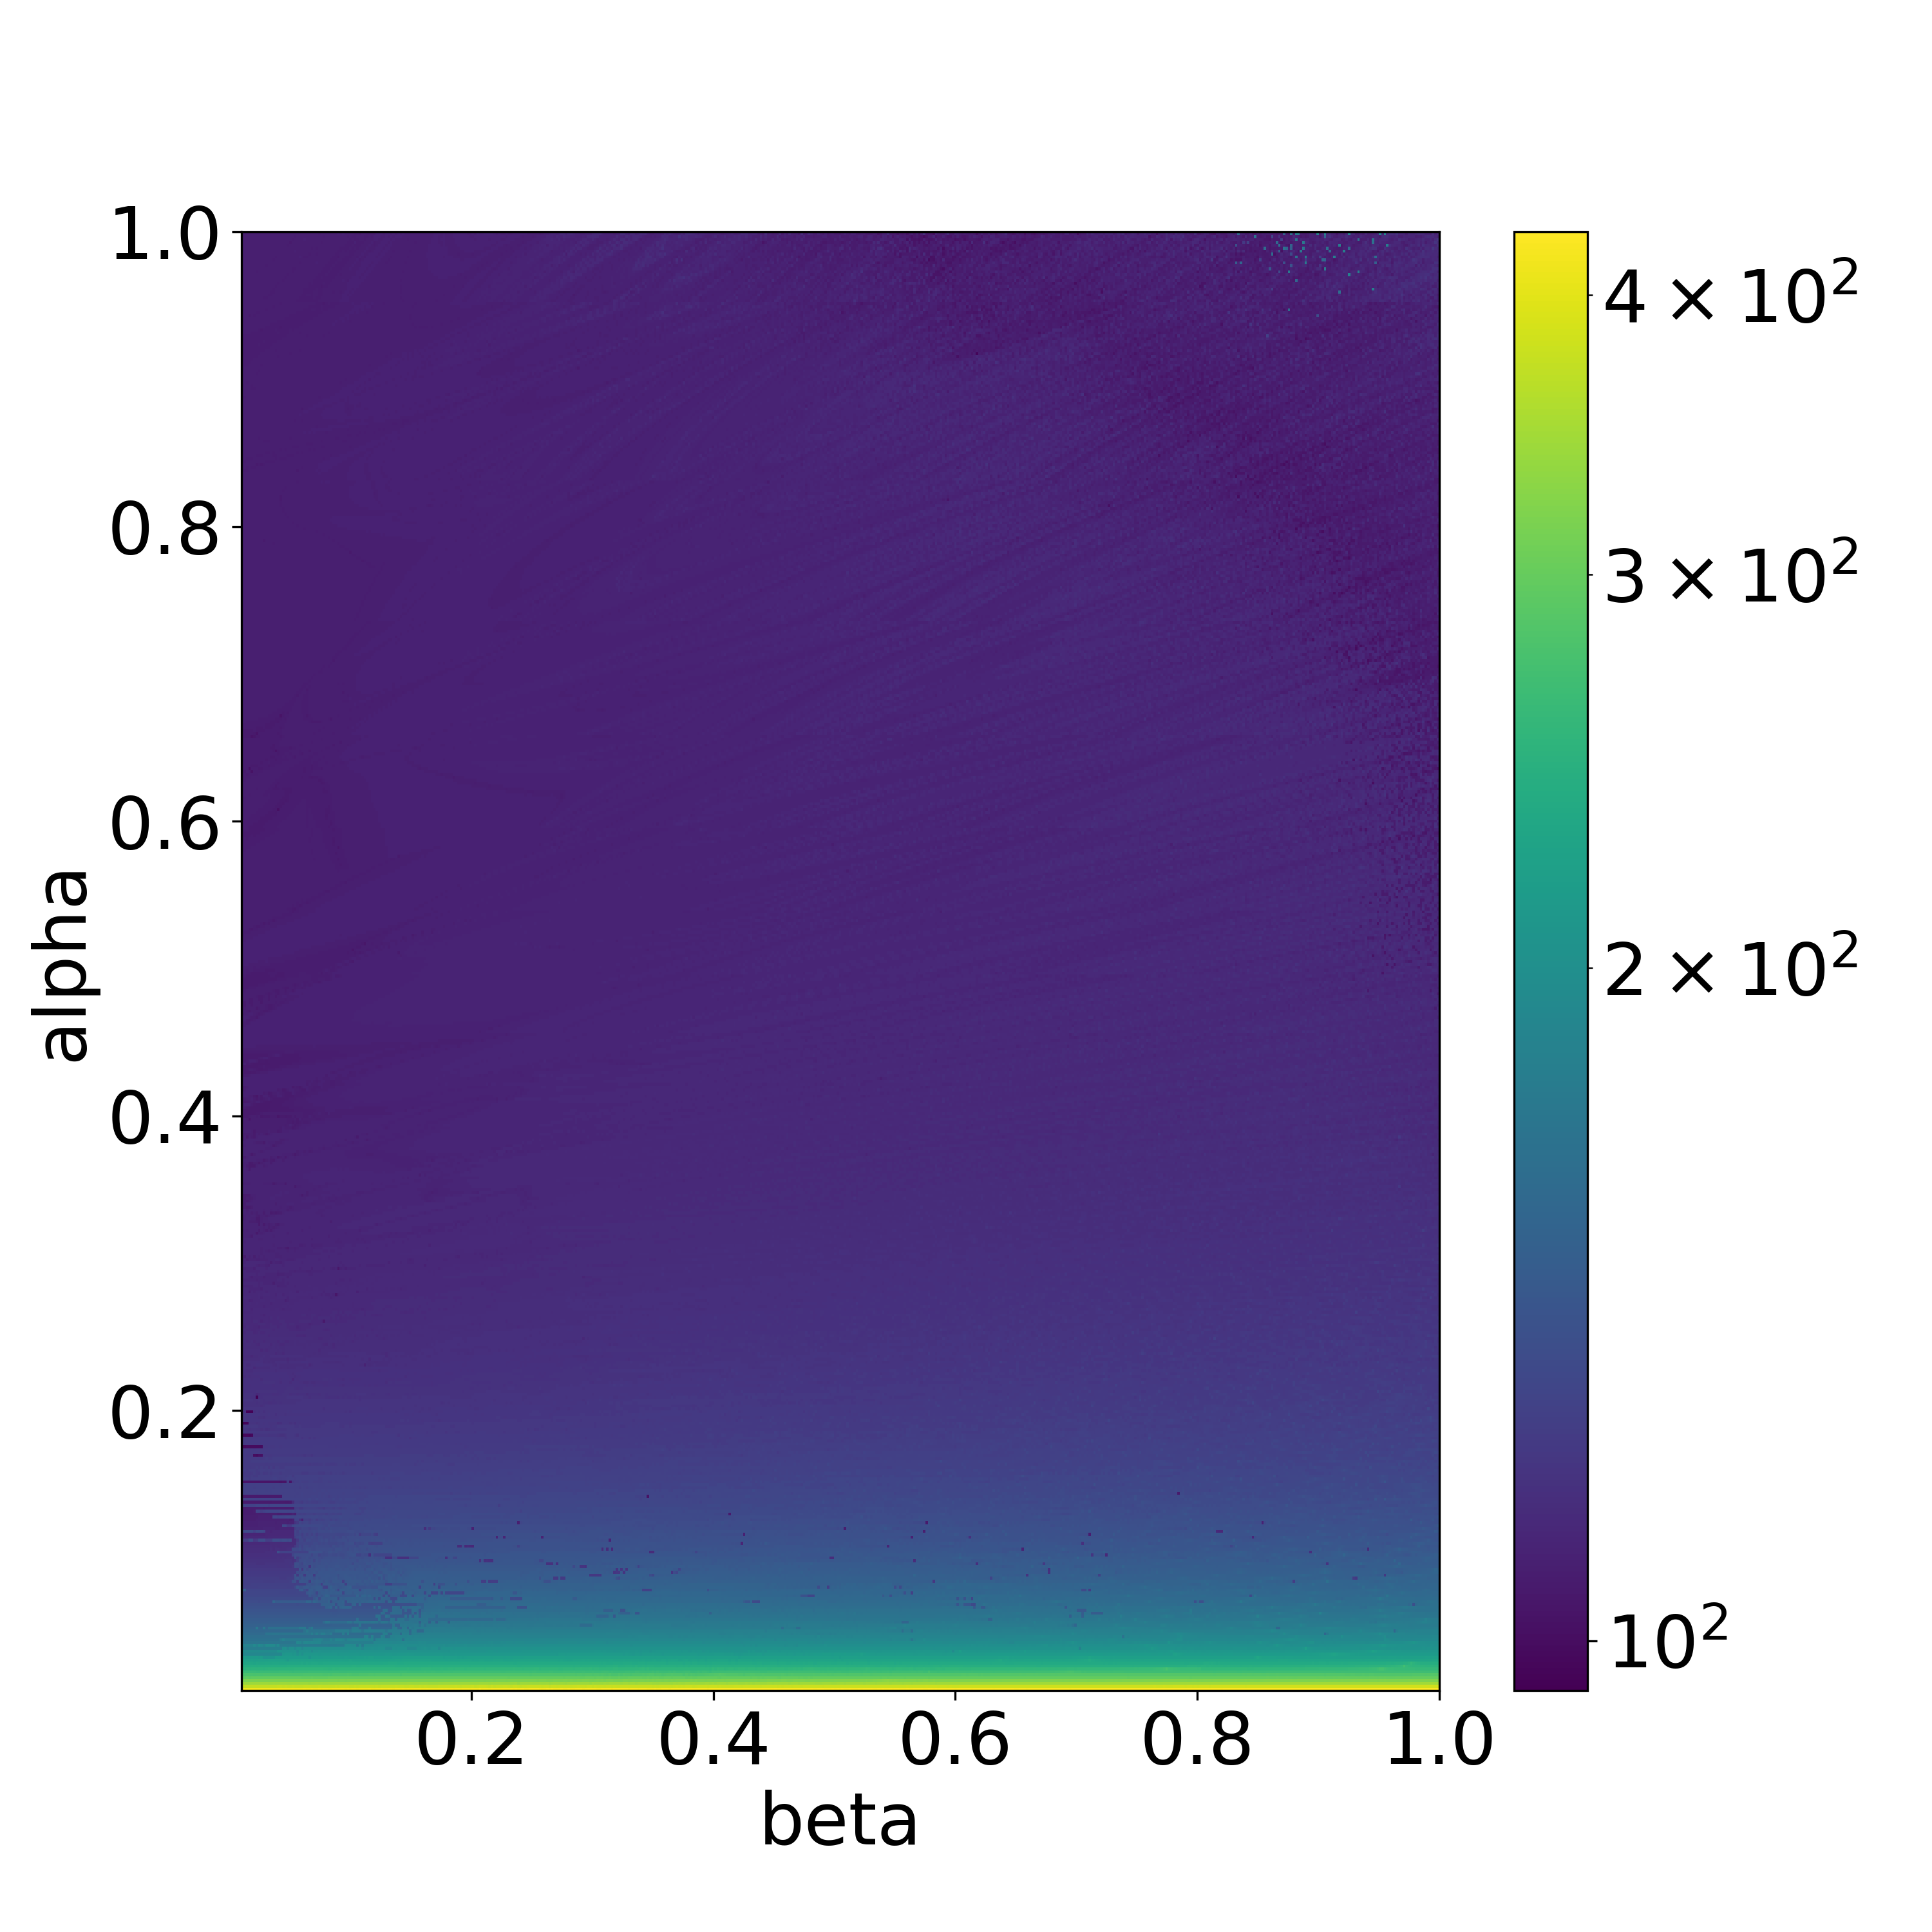
\includegraphics[width=1\textwidth]{images/analysis_RKF45_TS.png}
       	\subcaption{Number of required timesteps} 
        \label{fig:numberTimeStepsRKF45}
    \end{subfigure}
    \begin{subfigure}{0.32\textwidth}
    	\centering
    	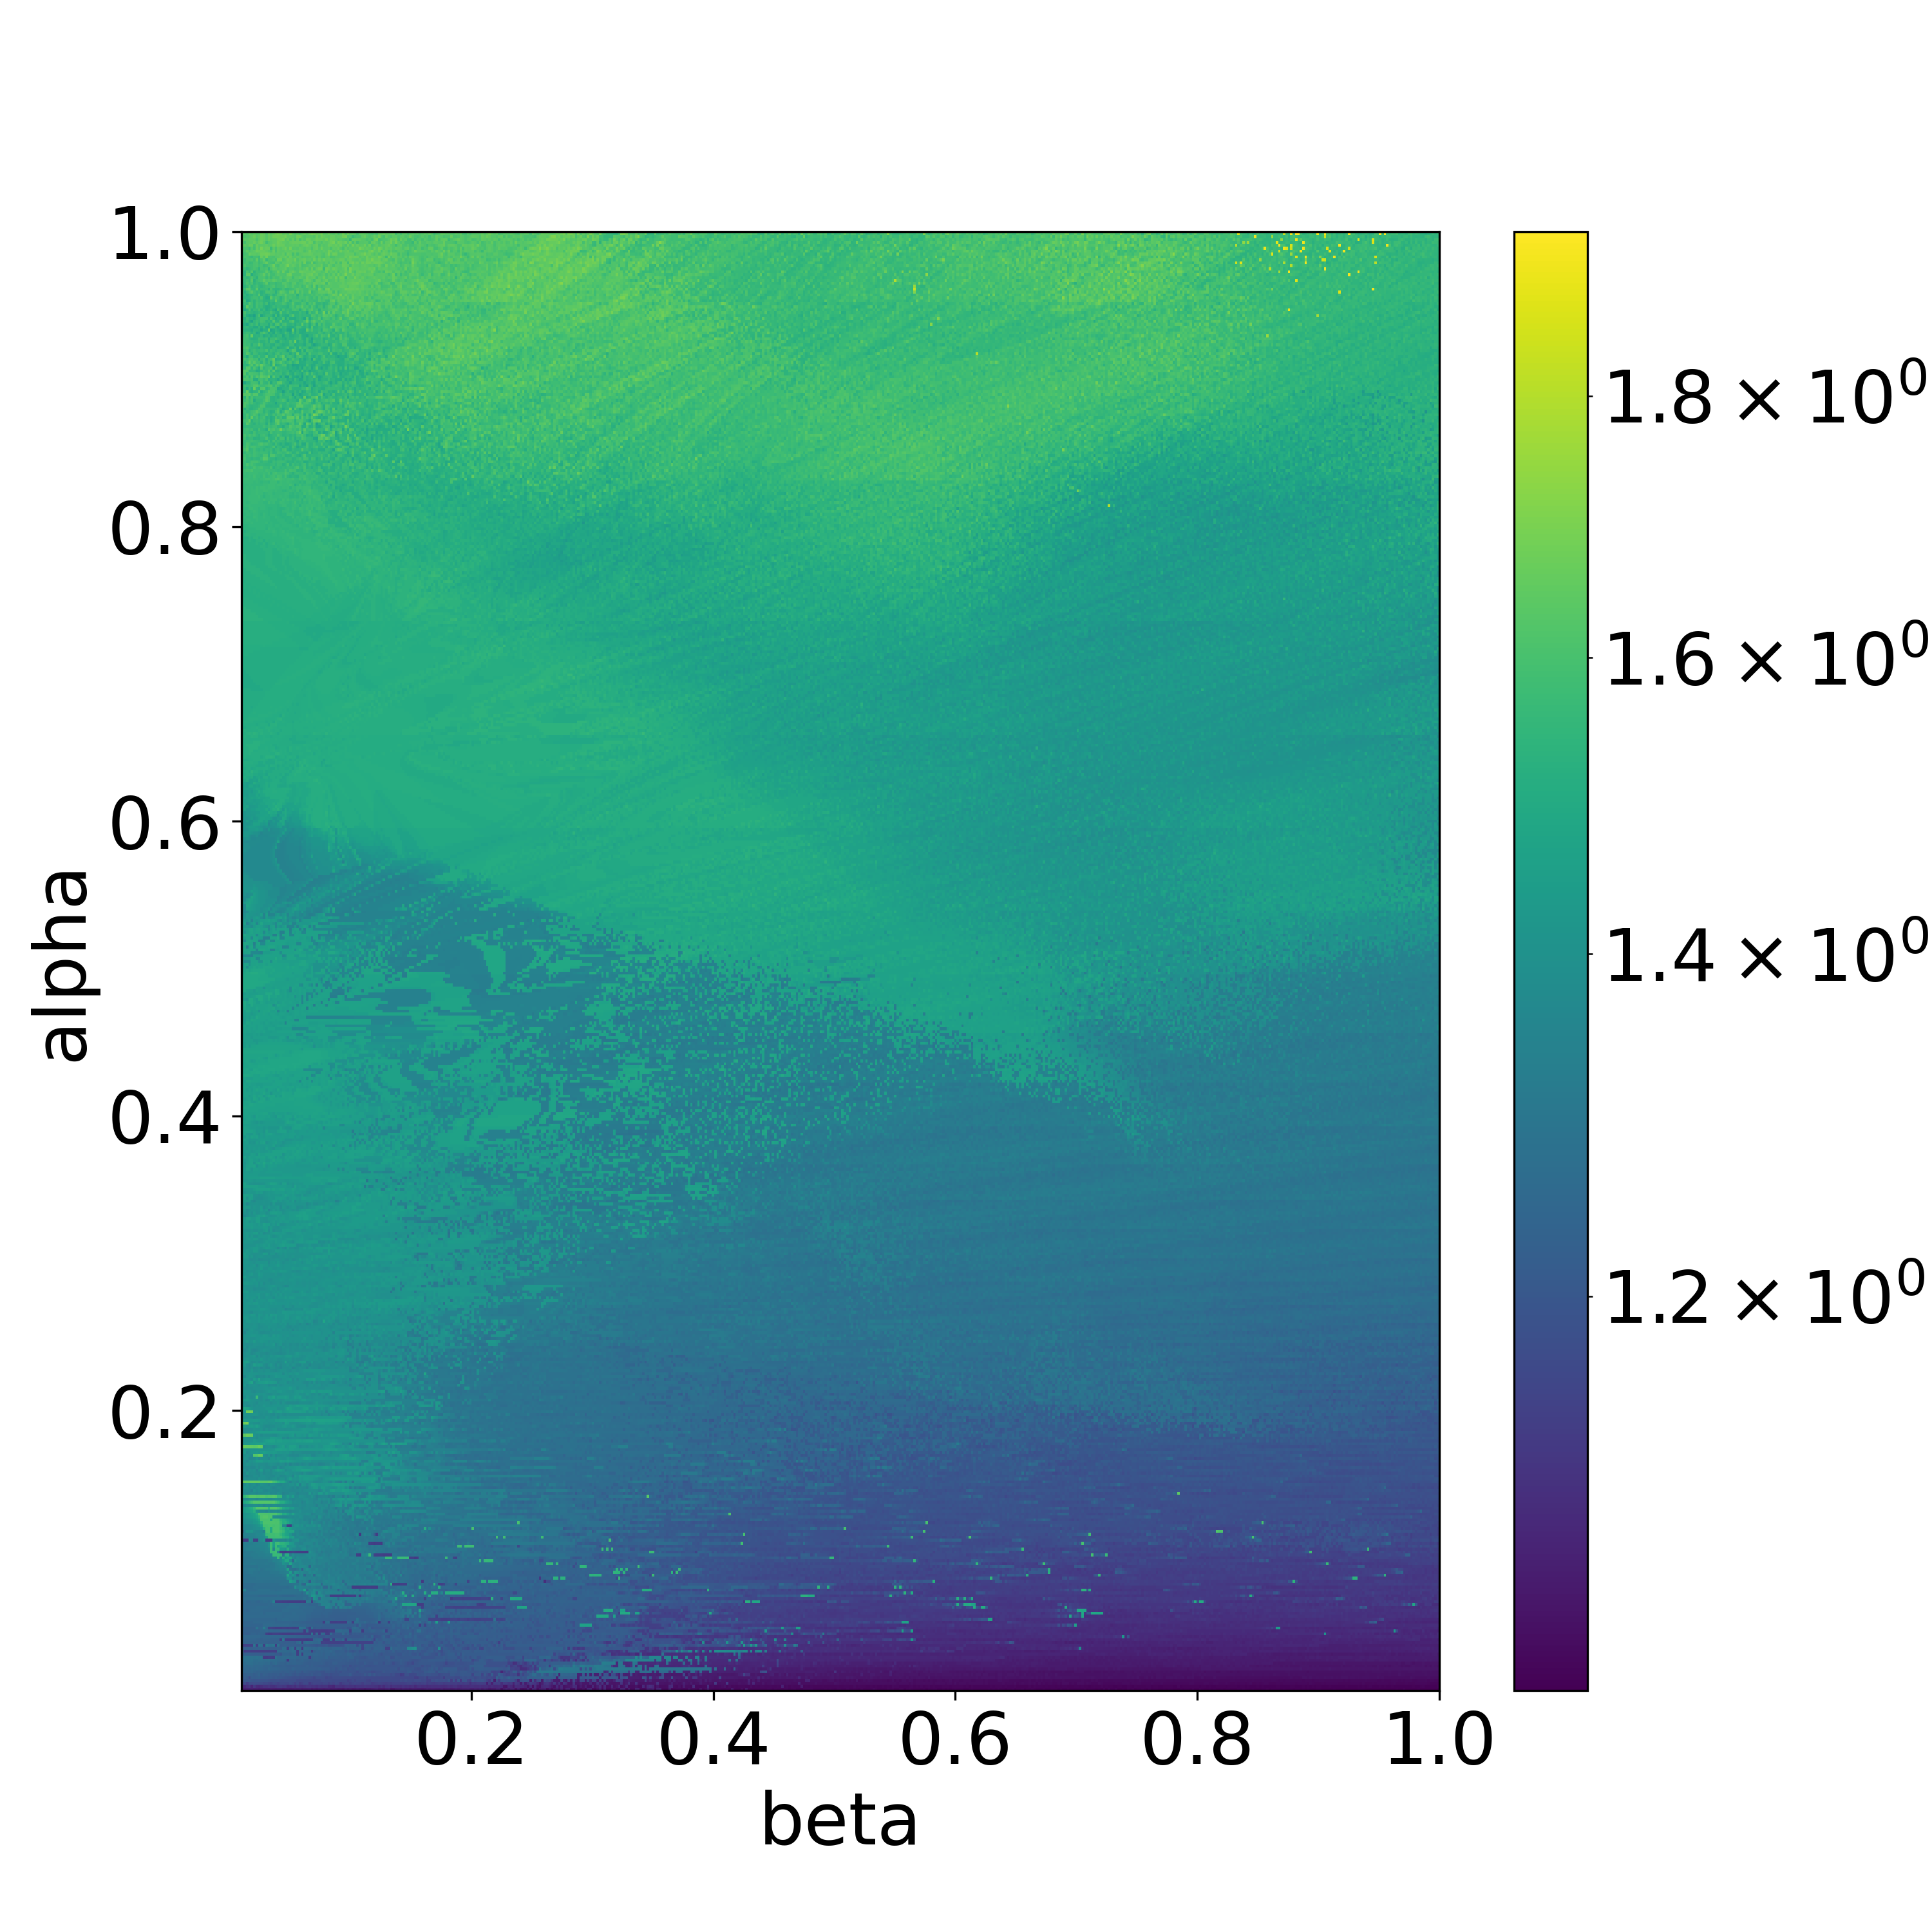
\includegraphics[width=1\textwidth]{images/analysis_RKF45_NI.png}
       	\subcaption{Average number of iterations per timestep} 
        \label{fig:numberIterationTSRKF45}
    \end{subfigure}
    \begin{subfigure}{0.32\textwidth}
    	\centering
    	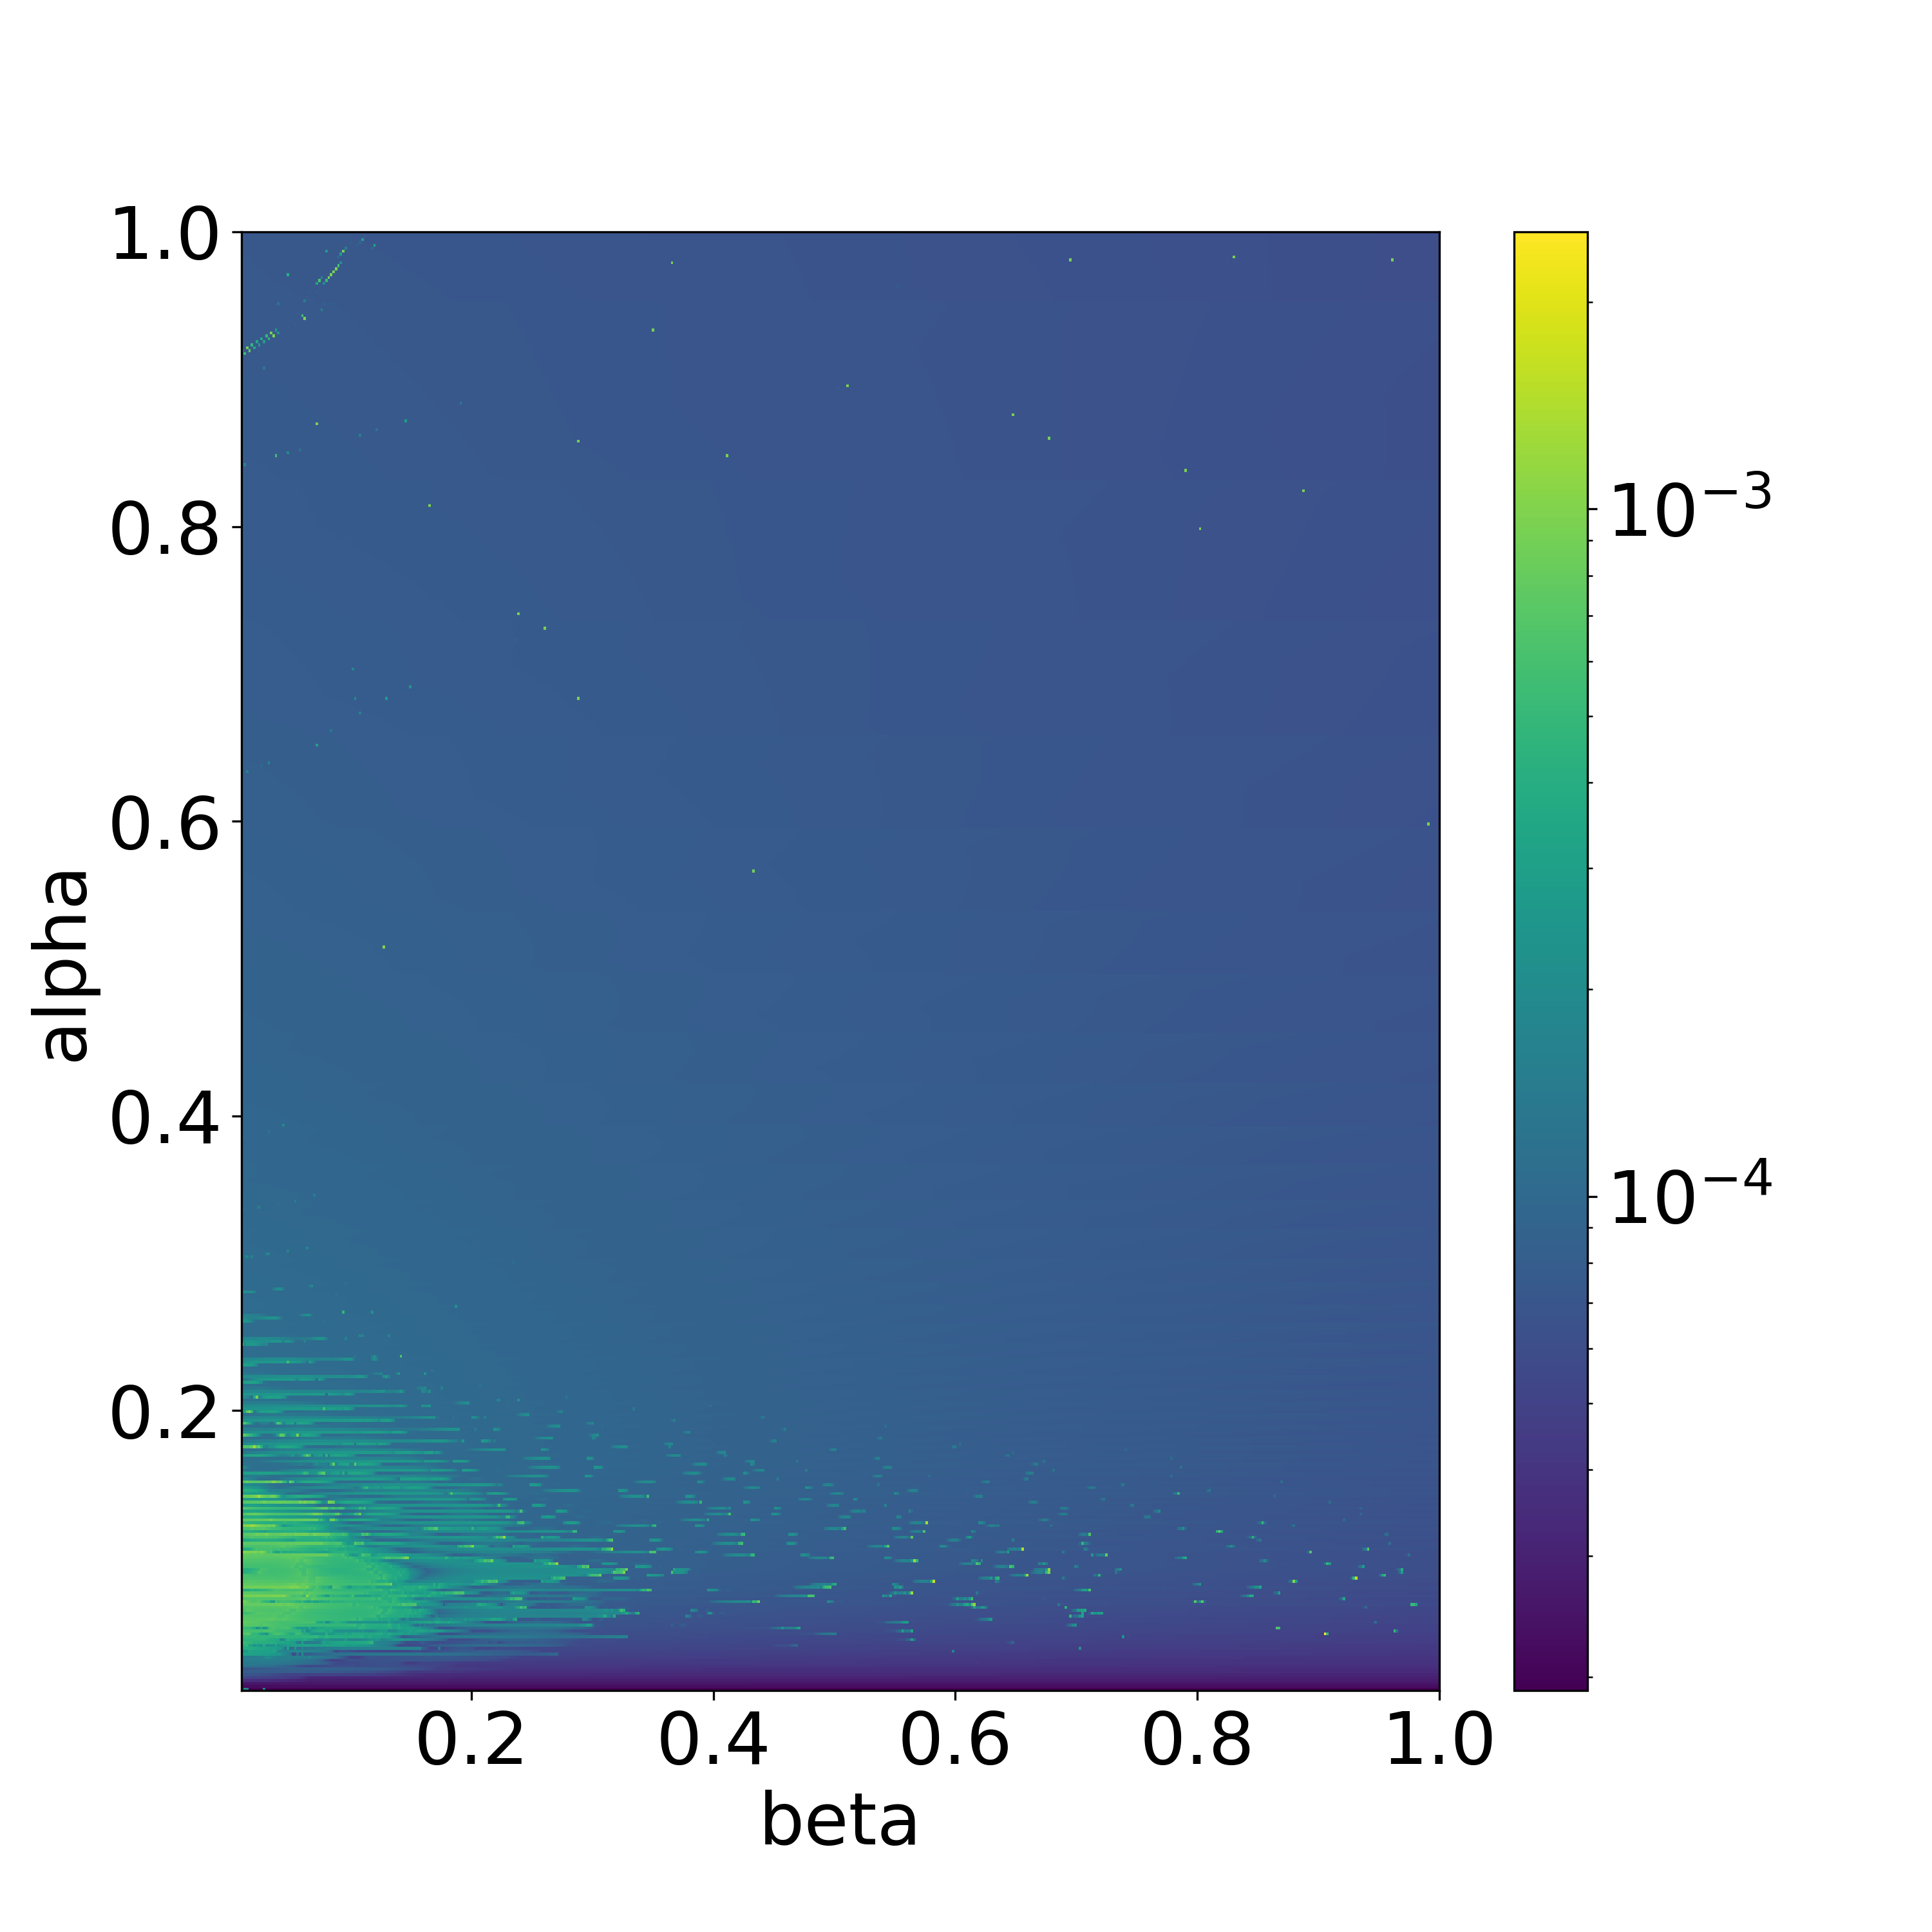
\includegraphics[width=1\textwidth]{images/analysis_RKF45_psi.png}
       	\subcaption{Absolute error of the variable $\psi$} 
        \label{fig:numberNumericalSchemeRKF45}
    \end{subfigure}
    \caption{Impact of the parameters $\alpha$ and $\beta$ of the PI controller on the number of required iterations to solve the model problem from \autoref{eq:first_DAE_ODE} using the explicit Runge-Kutta-Fehlberg method (\textbf{RKF45}) for a simulation time of $t=5.0s$}
    \label{fig:ParametersPIControllerRKF45}
\end{figure}


\begin{figure}[H]
    \centering
    \begin{subfigure}{0.32\textwidth}
    	\centering
    	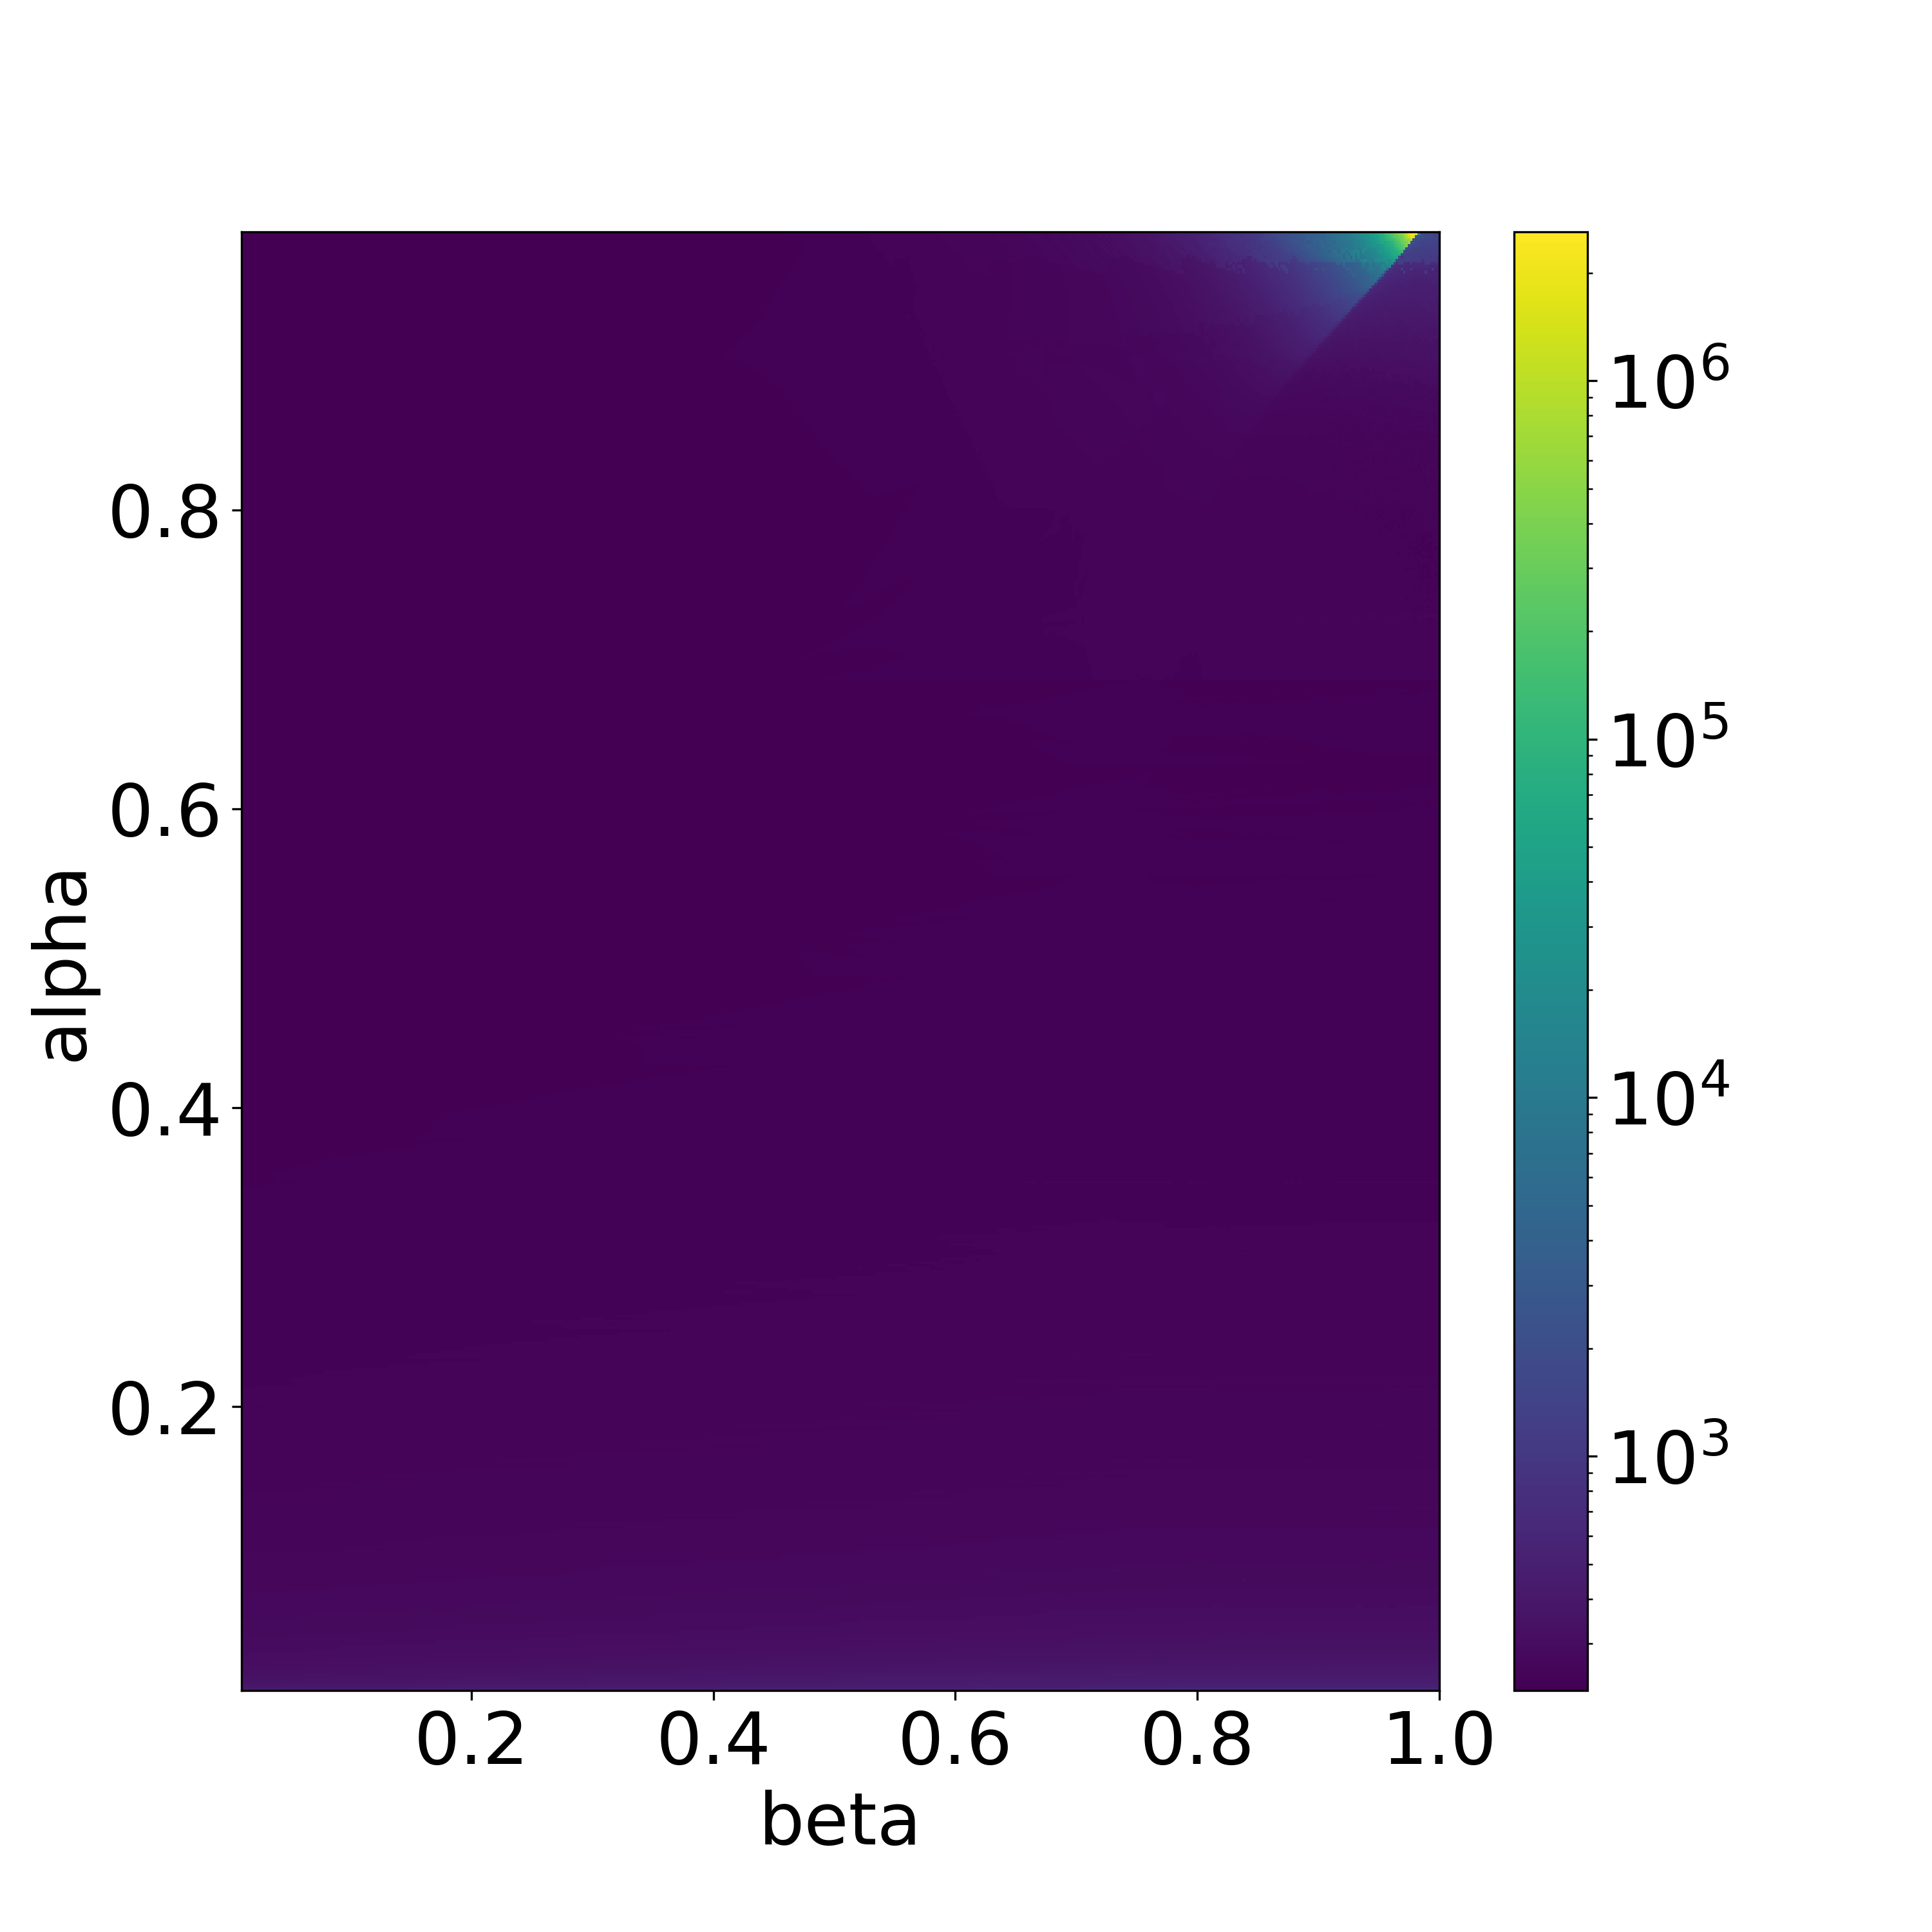
\includegraphics[width=1\textwidth]{images/analysis_BDF12_TS.png}
       	\subcaption{Number of required timesteps} 
        \label{fig:numberTimeStepsBDF12}
    \end{subfigure}
    \begin{subfigure}{0.32\textwidth}
    	\centering
    	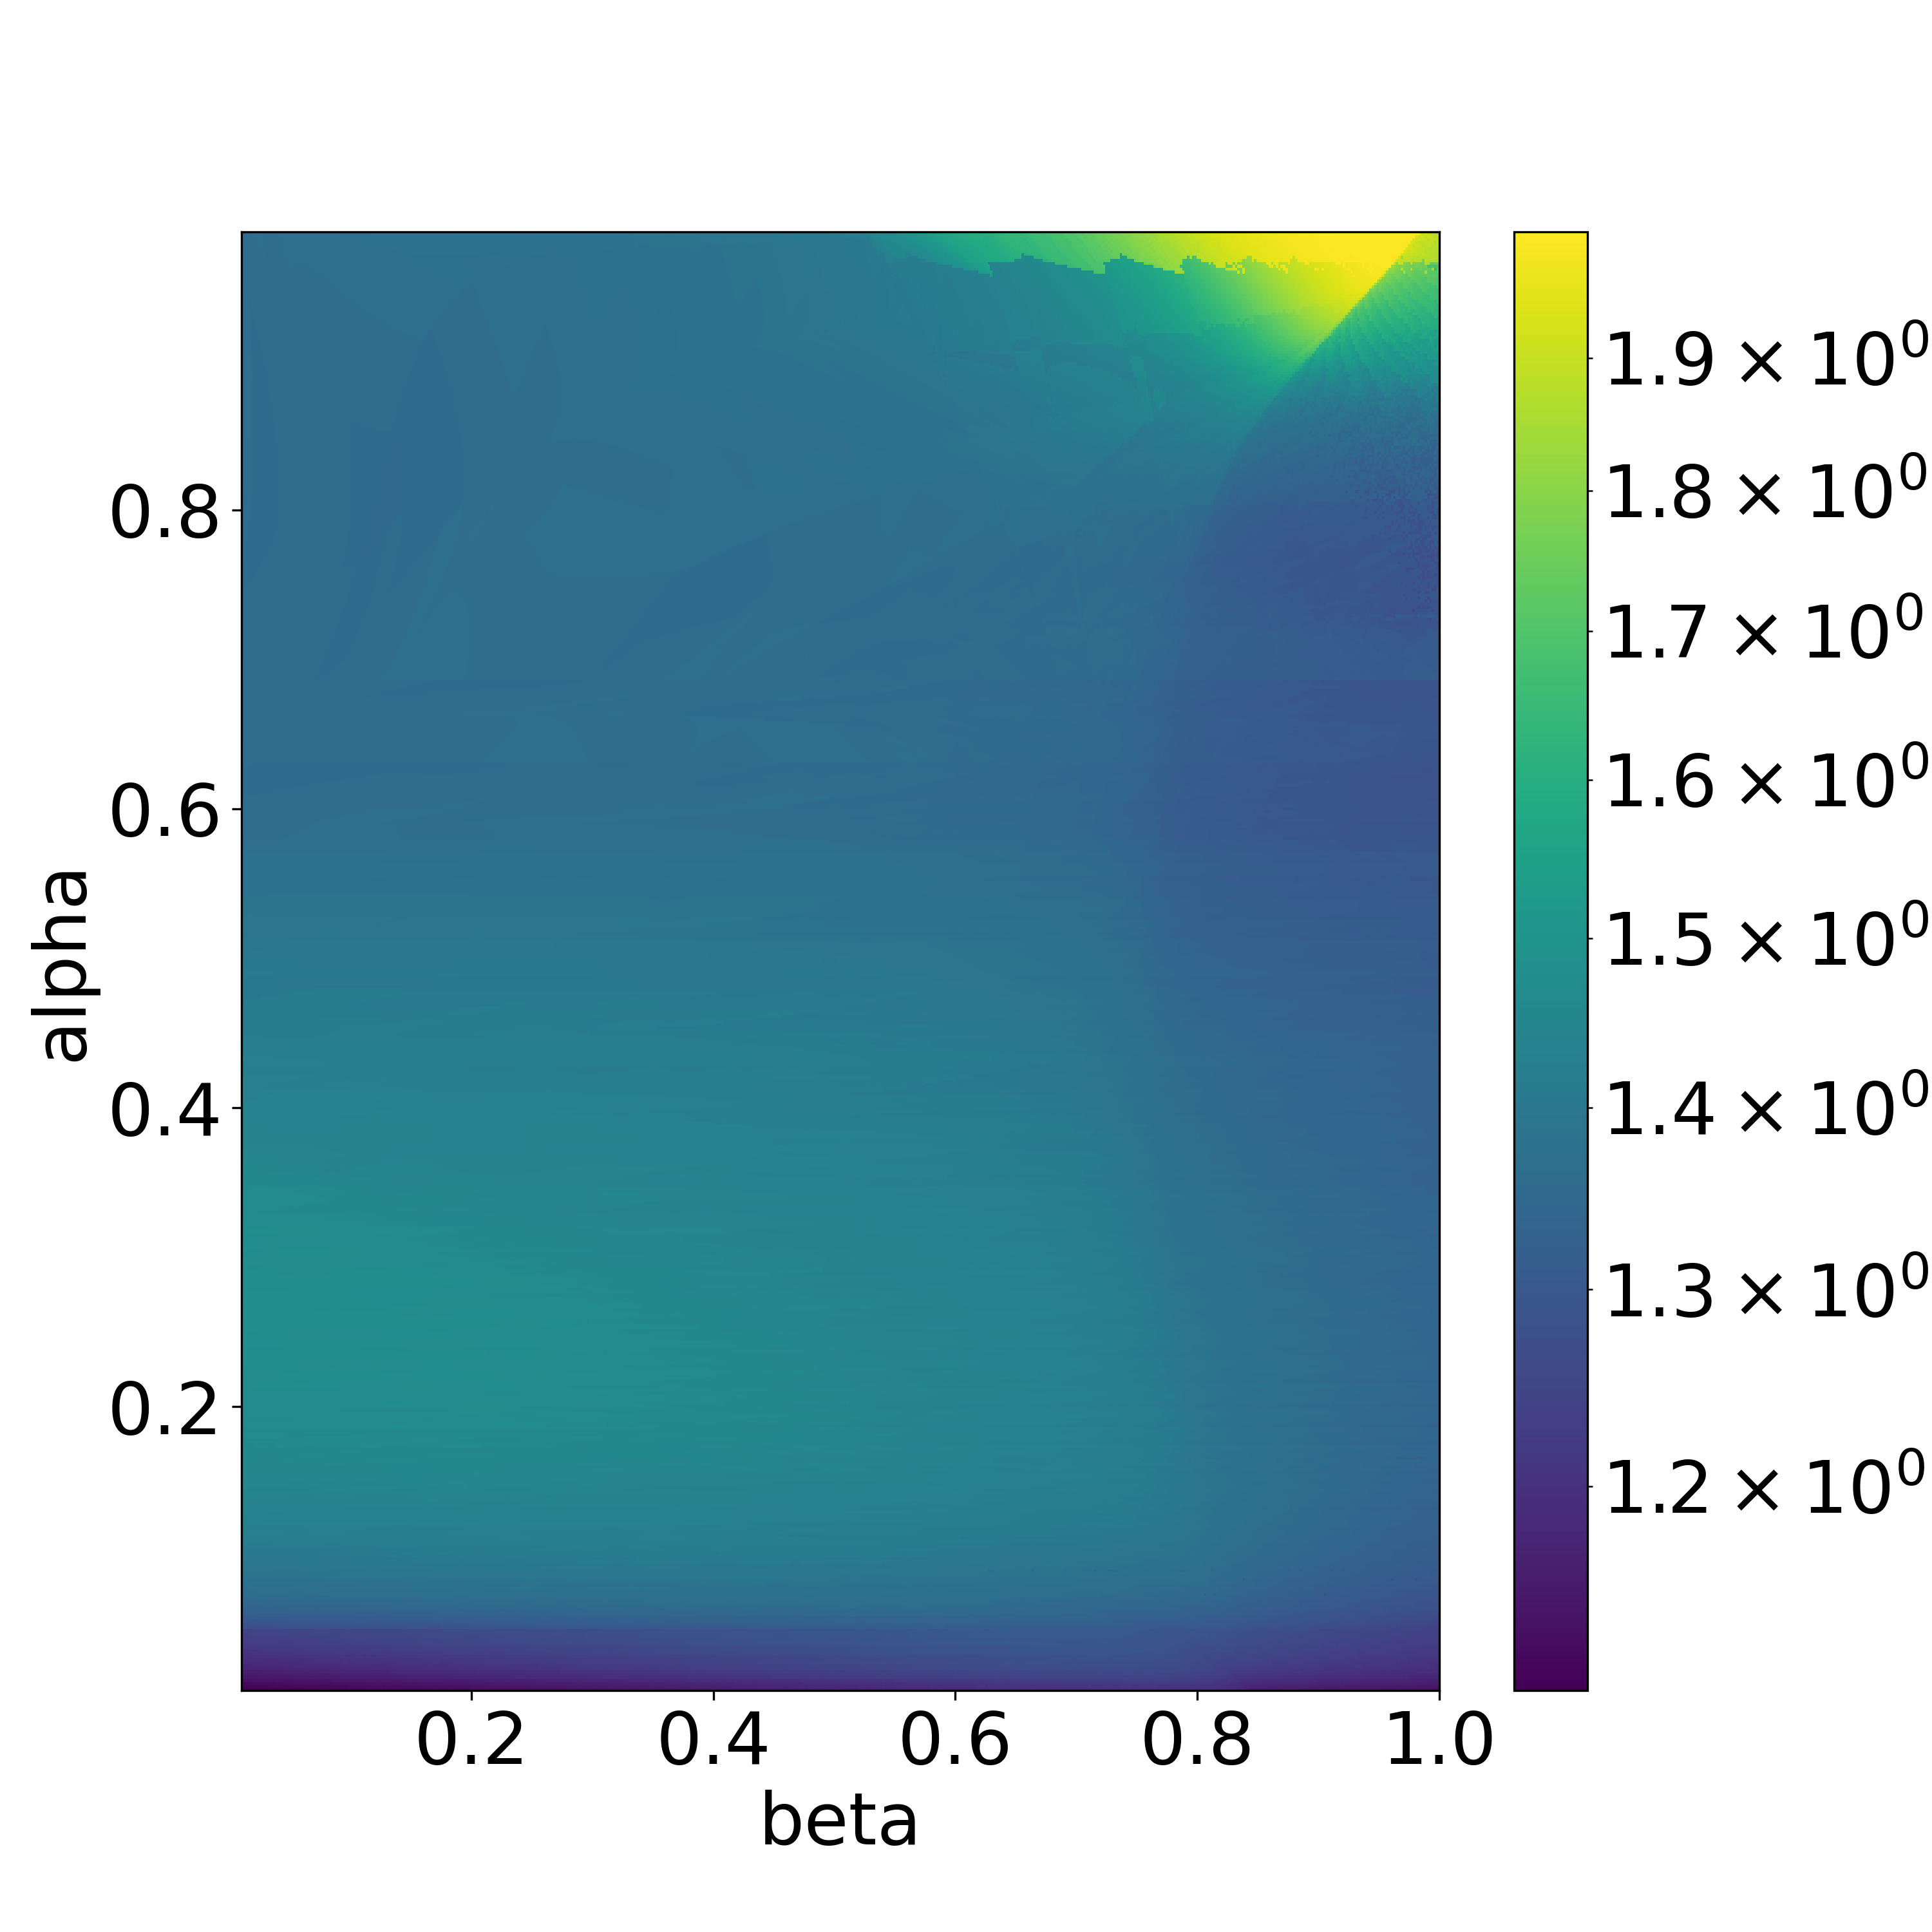
\includegraphics[width=1\textwidth]{images/analysis_BDF12_NI.png}
       	\subcaption{Average number of iterations per timestep} 
        \label{fig:numberIterationTSBDF12}
    \end{subfigure}
    \begin{subfigure}{0.32\textwidth}
    	\centering
    	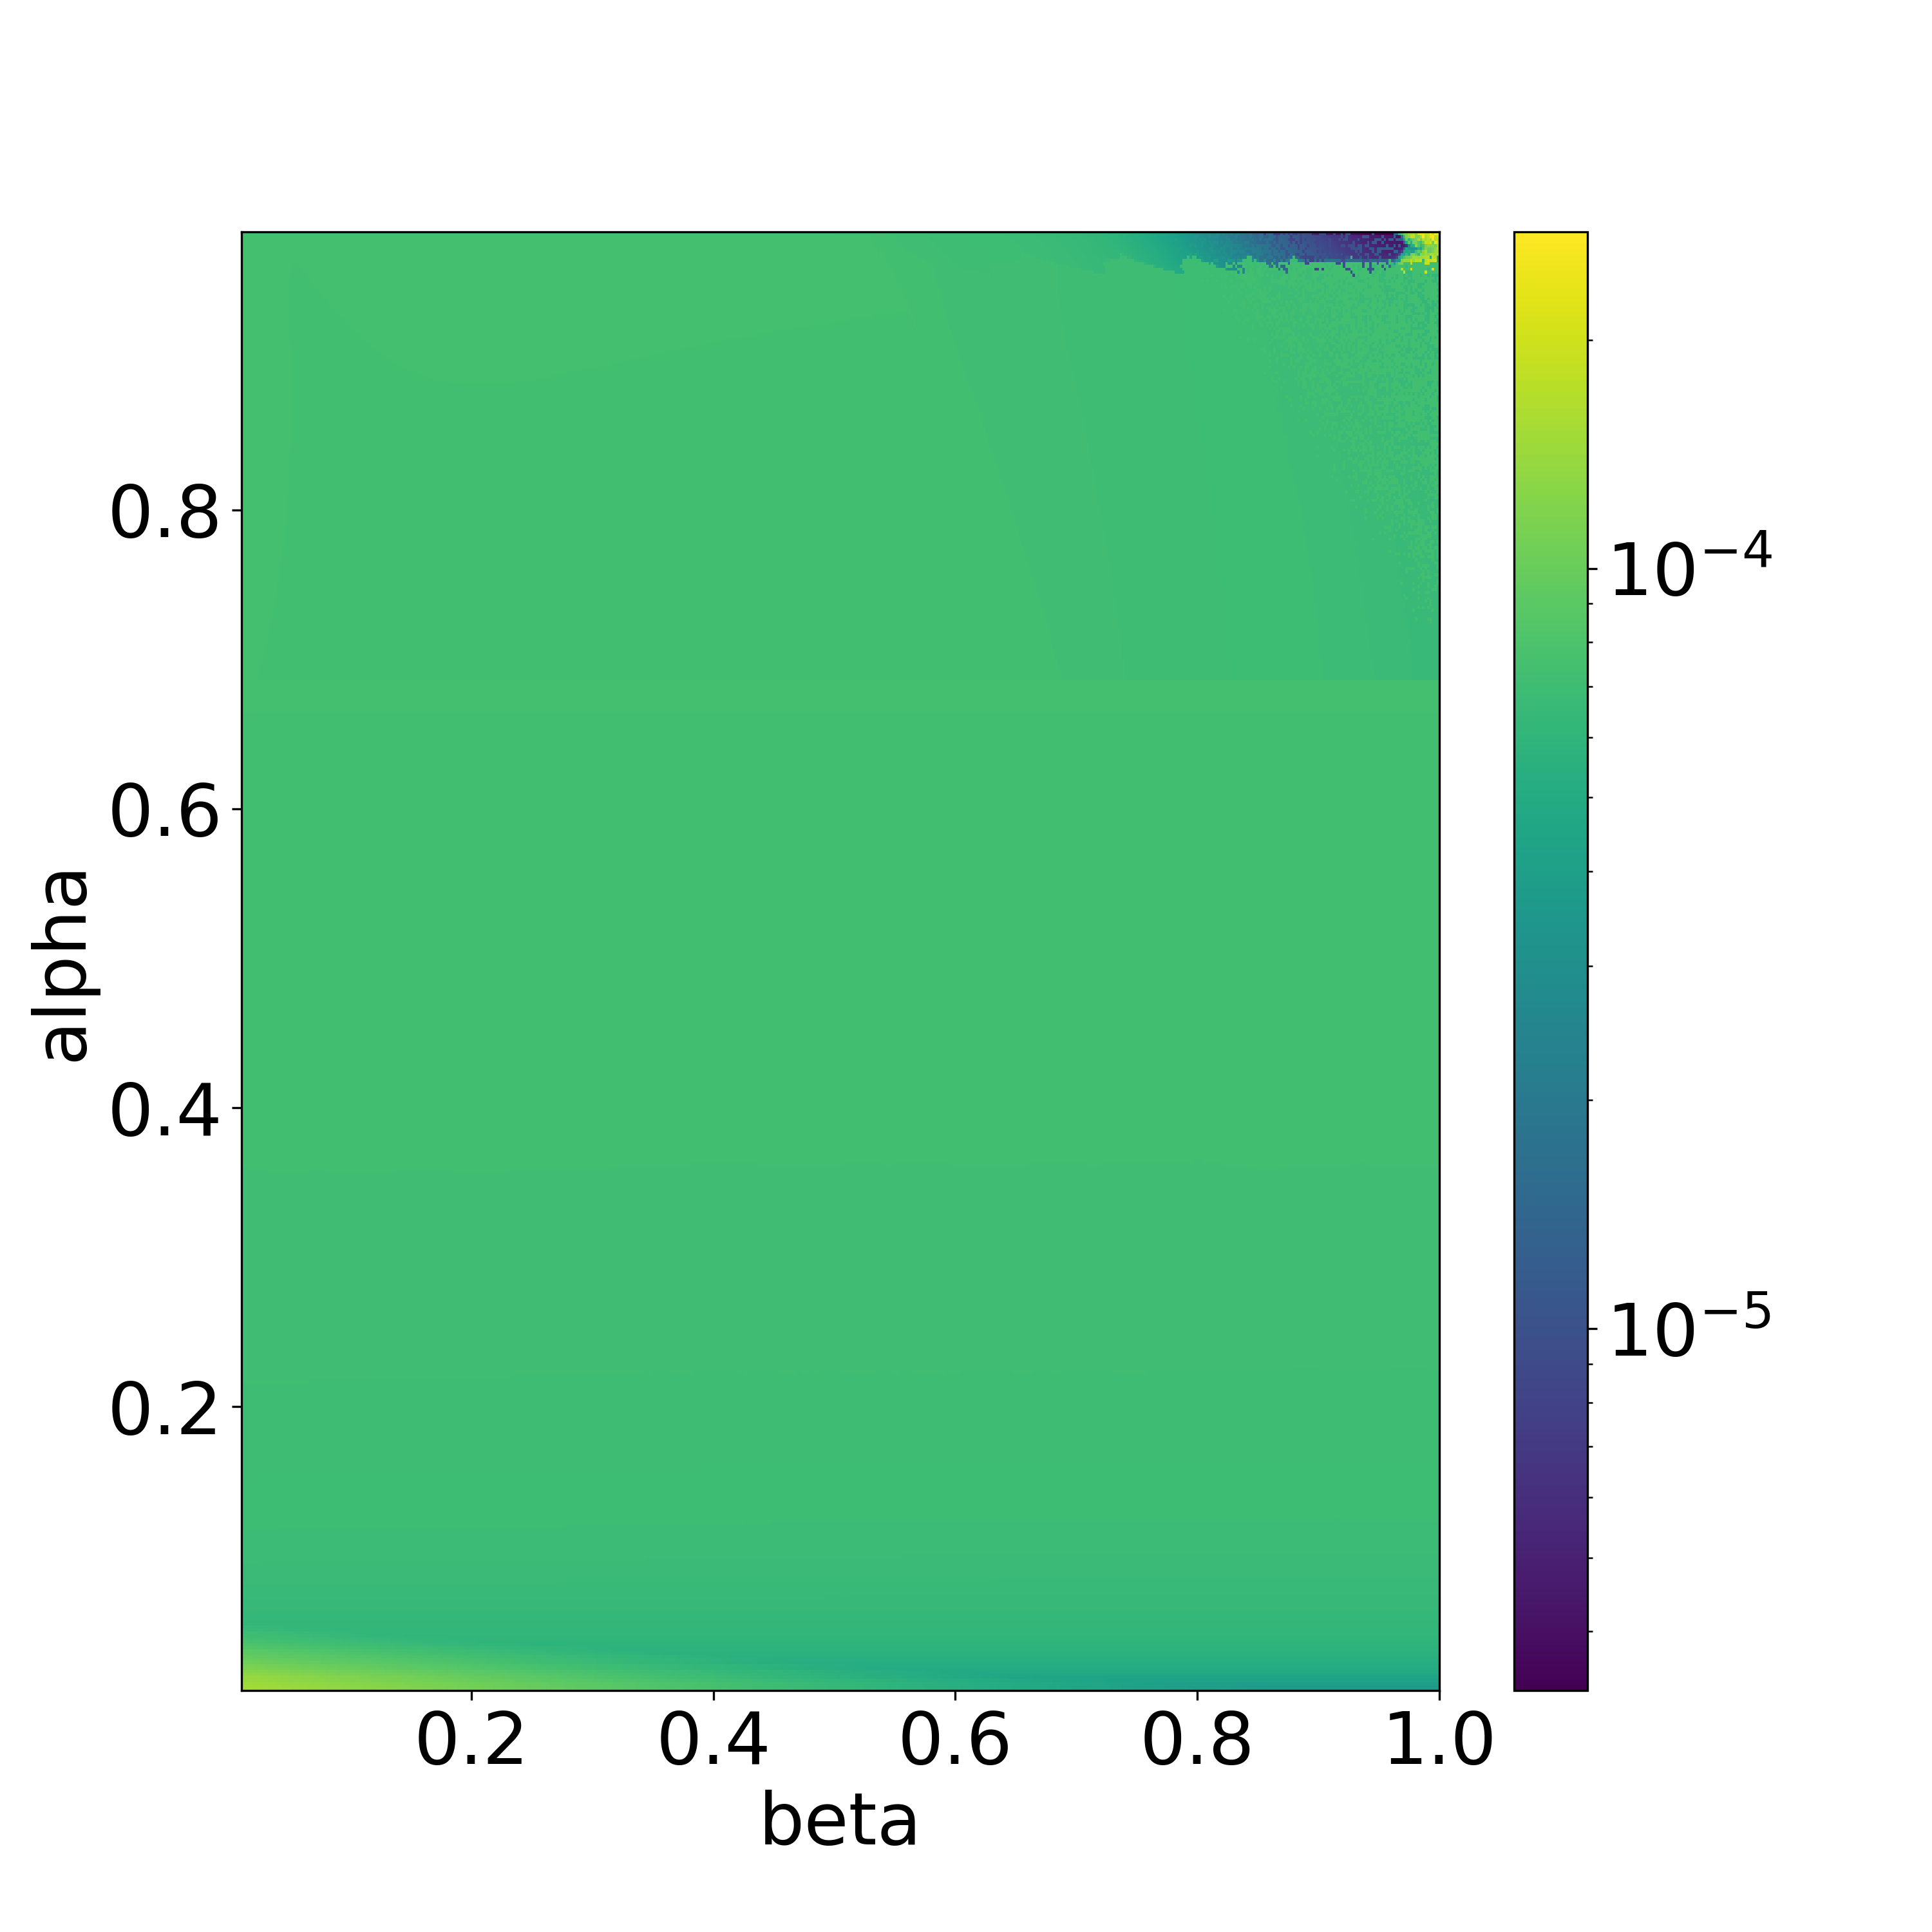
\includegraphics[width=1\textwidth]{images/analysis_BDF12_psi.png}
       	\subcaption{Absolute error of the variable $\psi$} 
        \label{fig:numberNumericalSchemeBDF12}
    \end{subfigure}
    \caption{Impact of the parameters $\alpha$ and $\beta$ of the PI controller on the number of required iterations to solve the model problem from \autoref{eq:first_DAE_ODE} using the implicit BDF method of first order (\textbf{BDF12}) for a simulation time of $t=5.0s$}
    \label{fig:ParametersPIControllerBDF12}
\end{figure}


\begin{figure}[H]
    \centering
    \begin{subfigure}{0.32\textwidth}
    	\centering
    	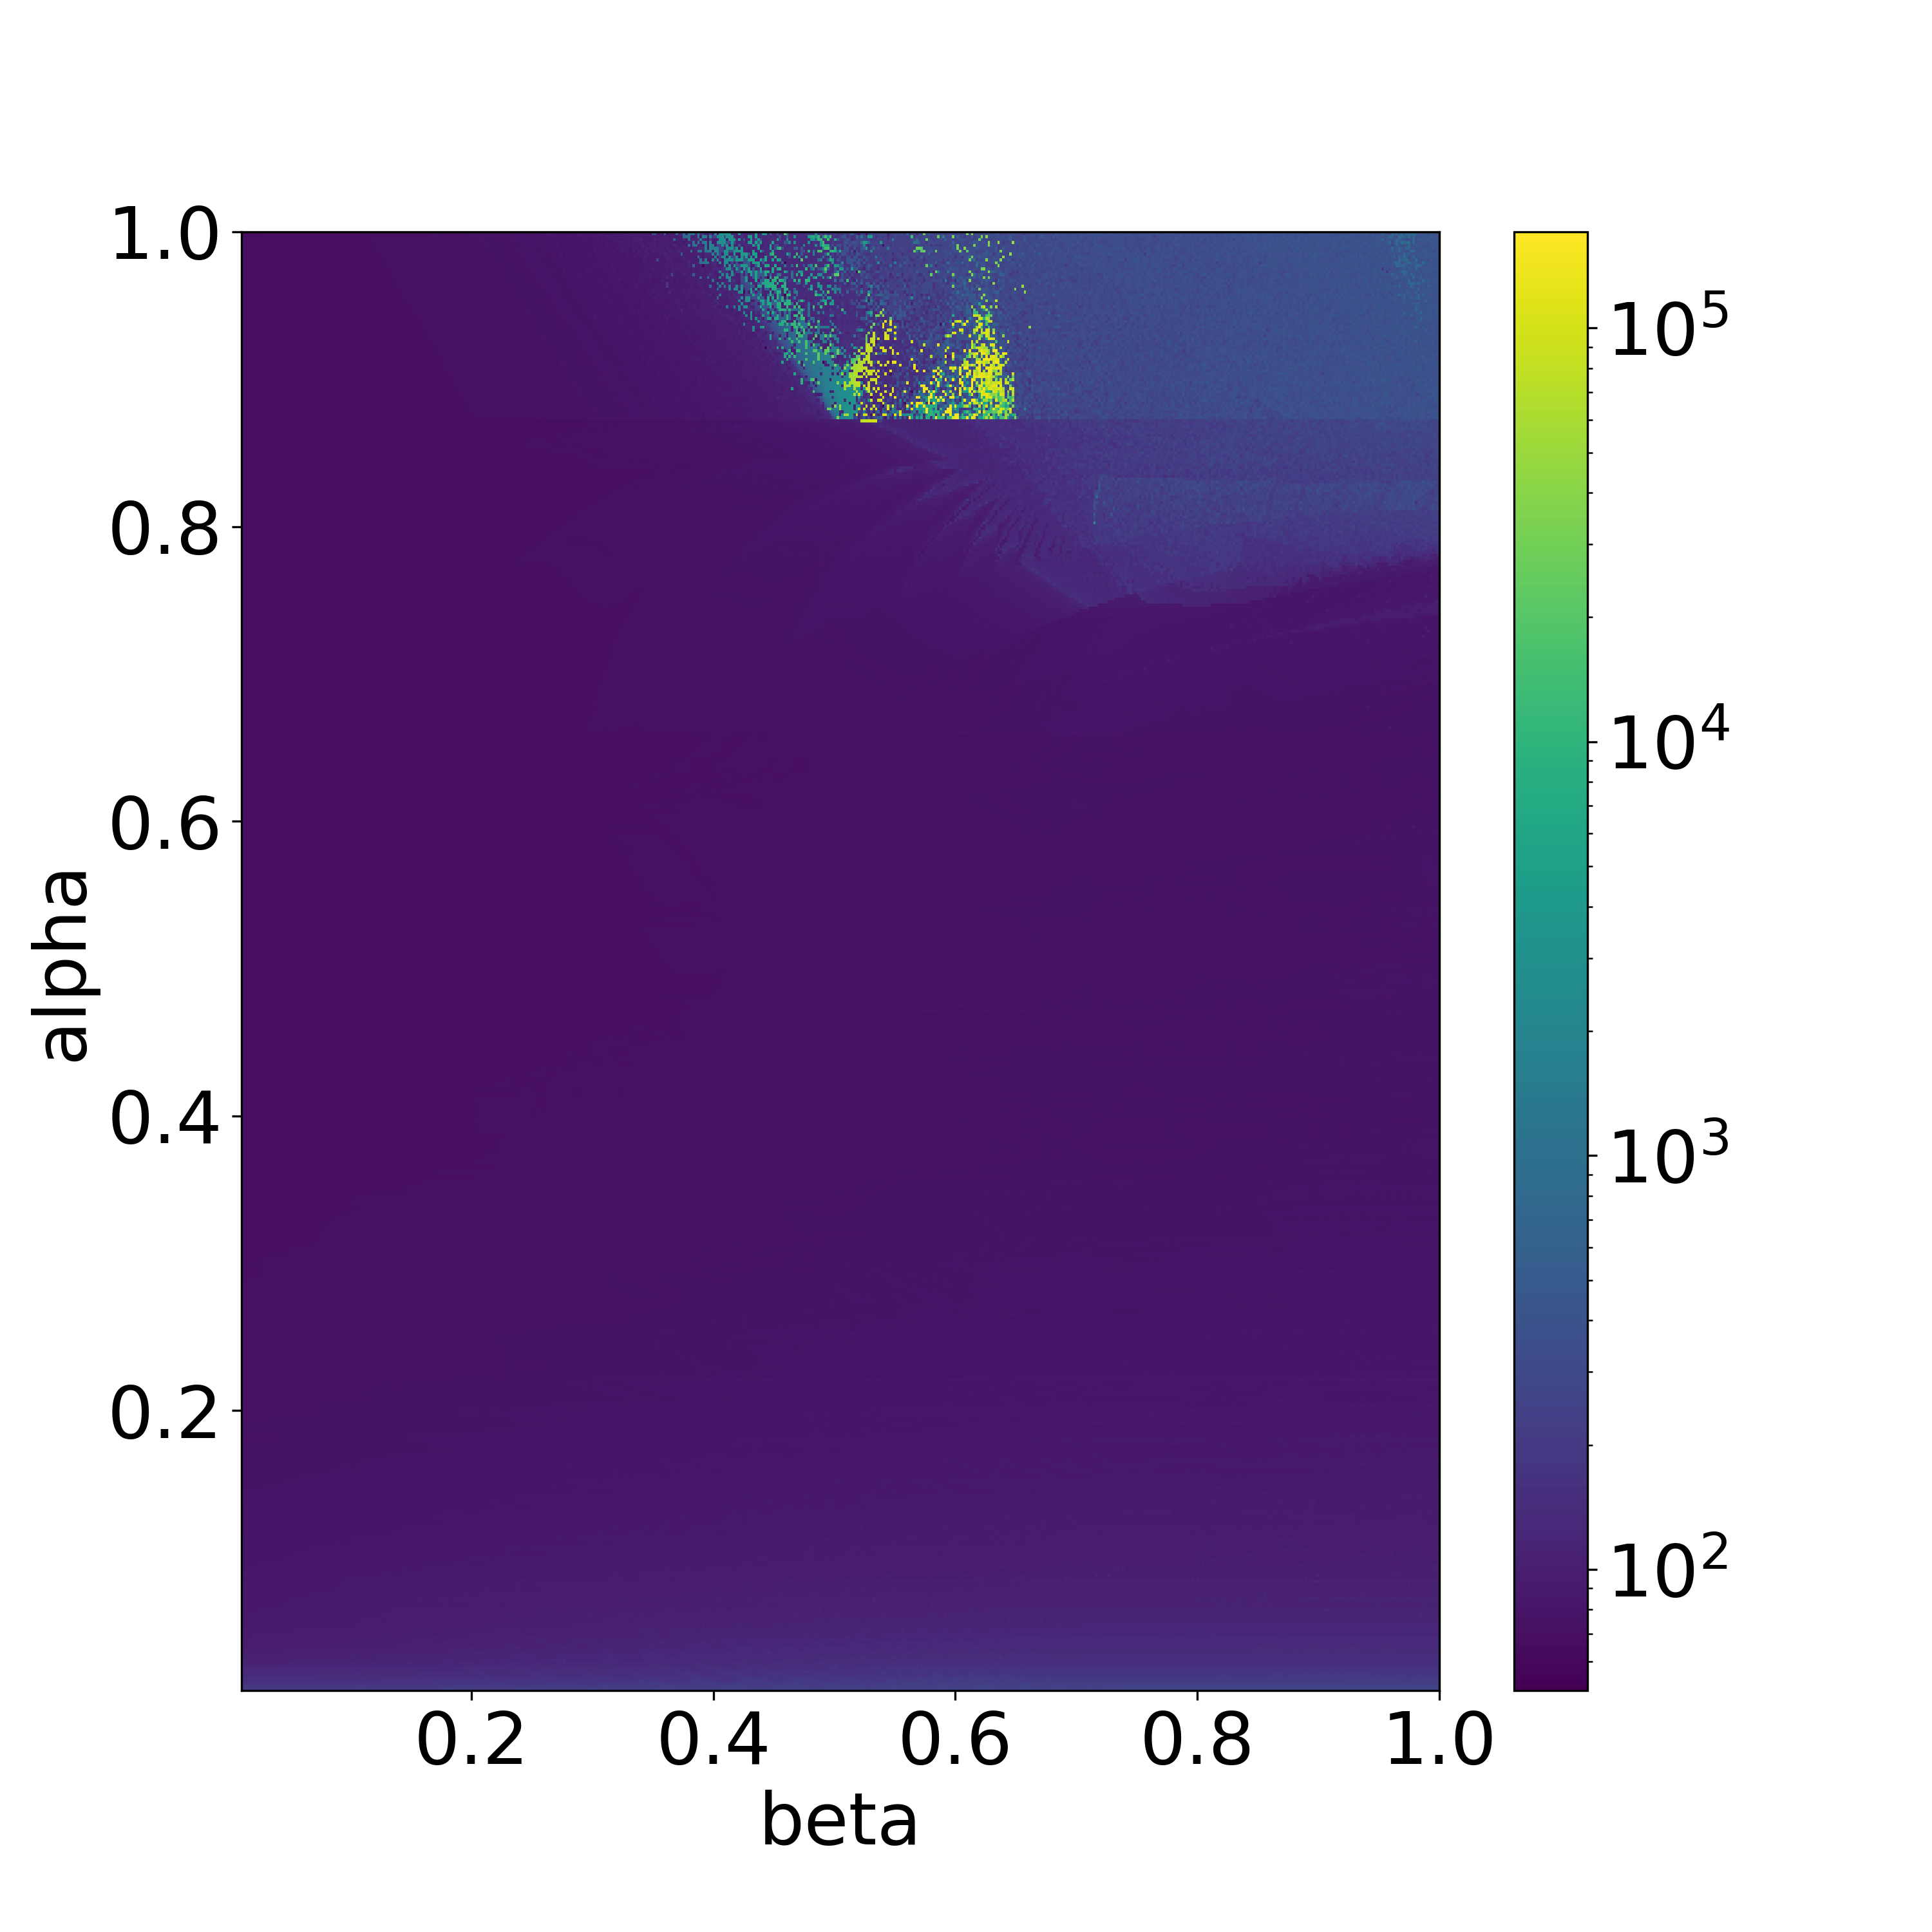
\includegraphics[width=1\textwidth]{images/analysis_BDF23_TS.png}
       	\subcaption{Number of required timesteps} 
        \label{fig:numberTimeStepsBDF23}
    \end{subfigure}
    \begin{subfigure}{0.32\textwidth}
    	\centering
    	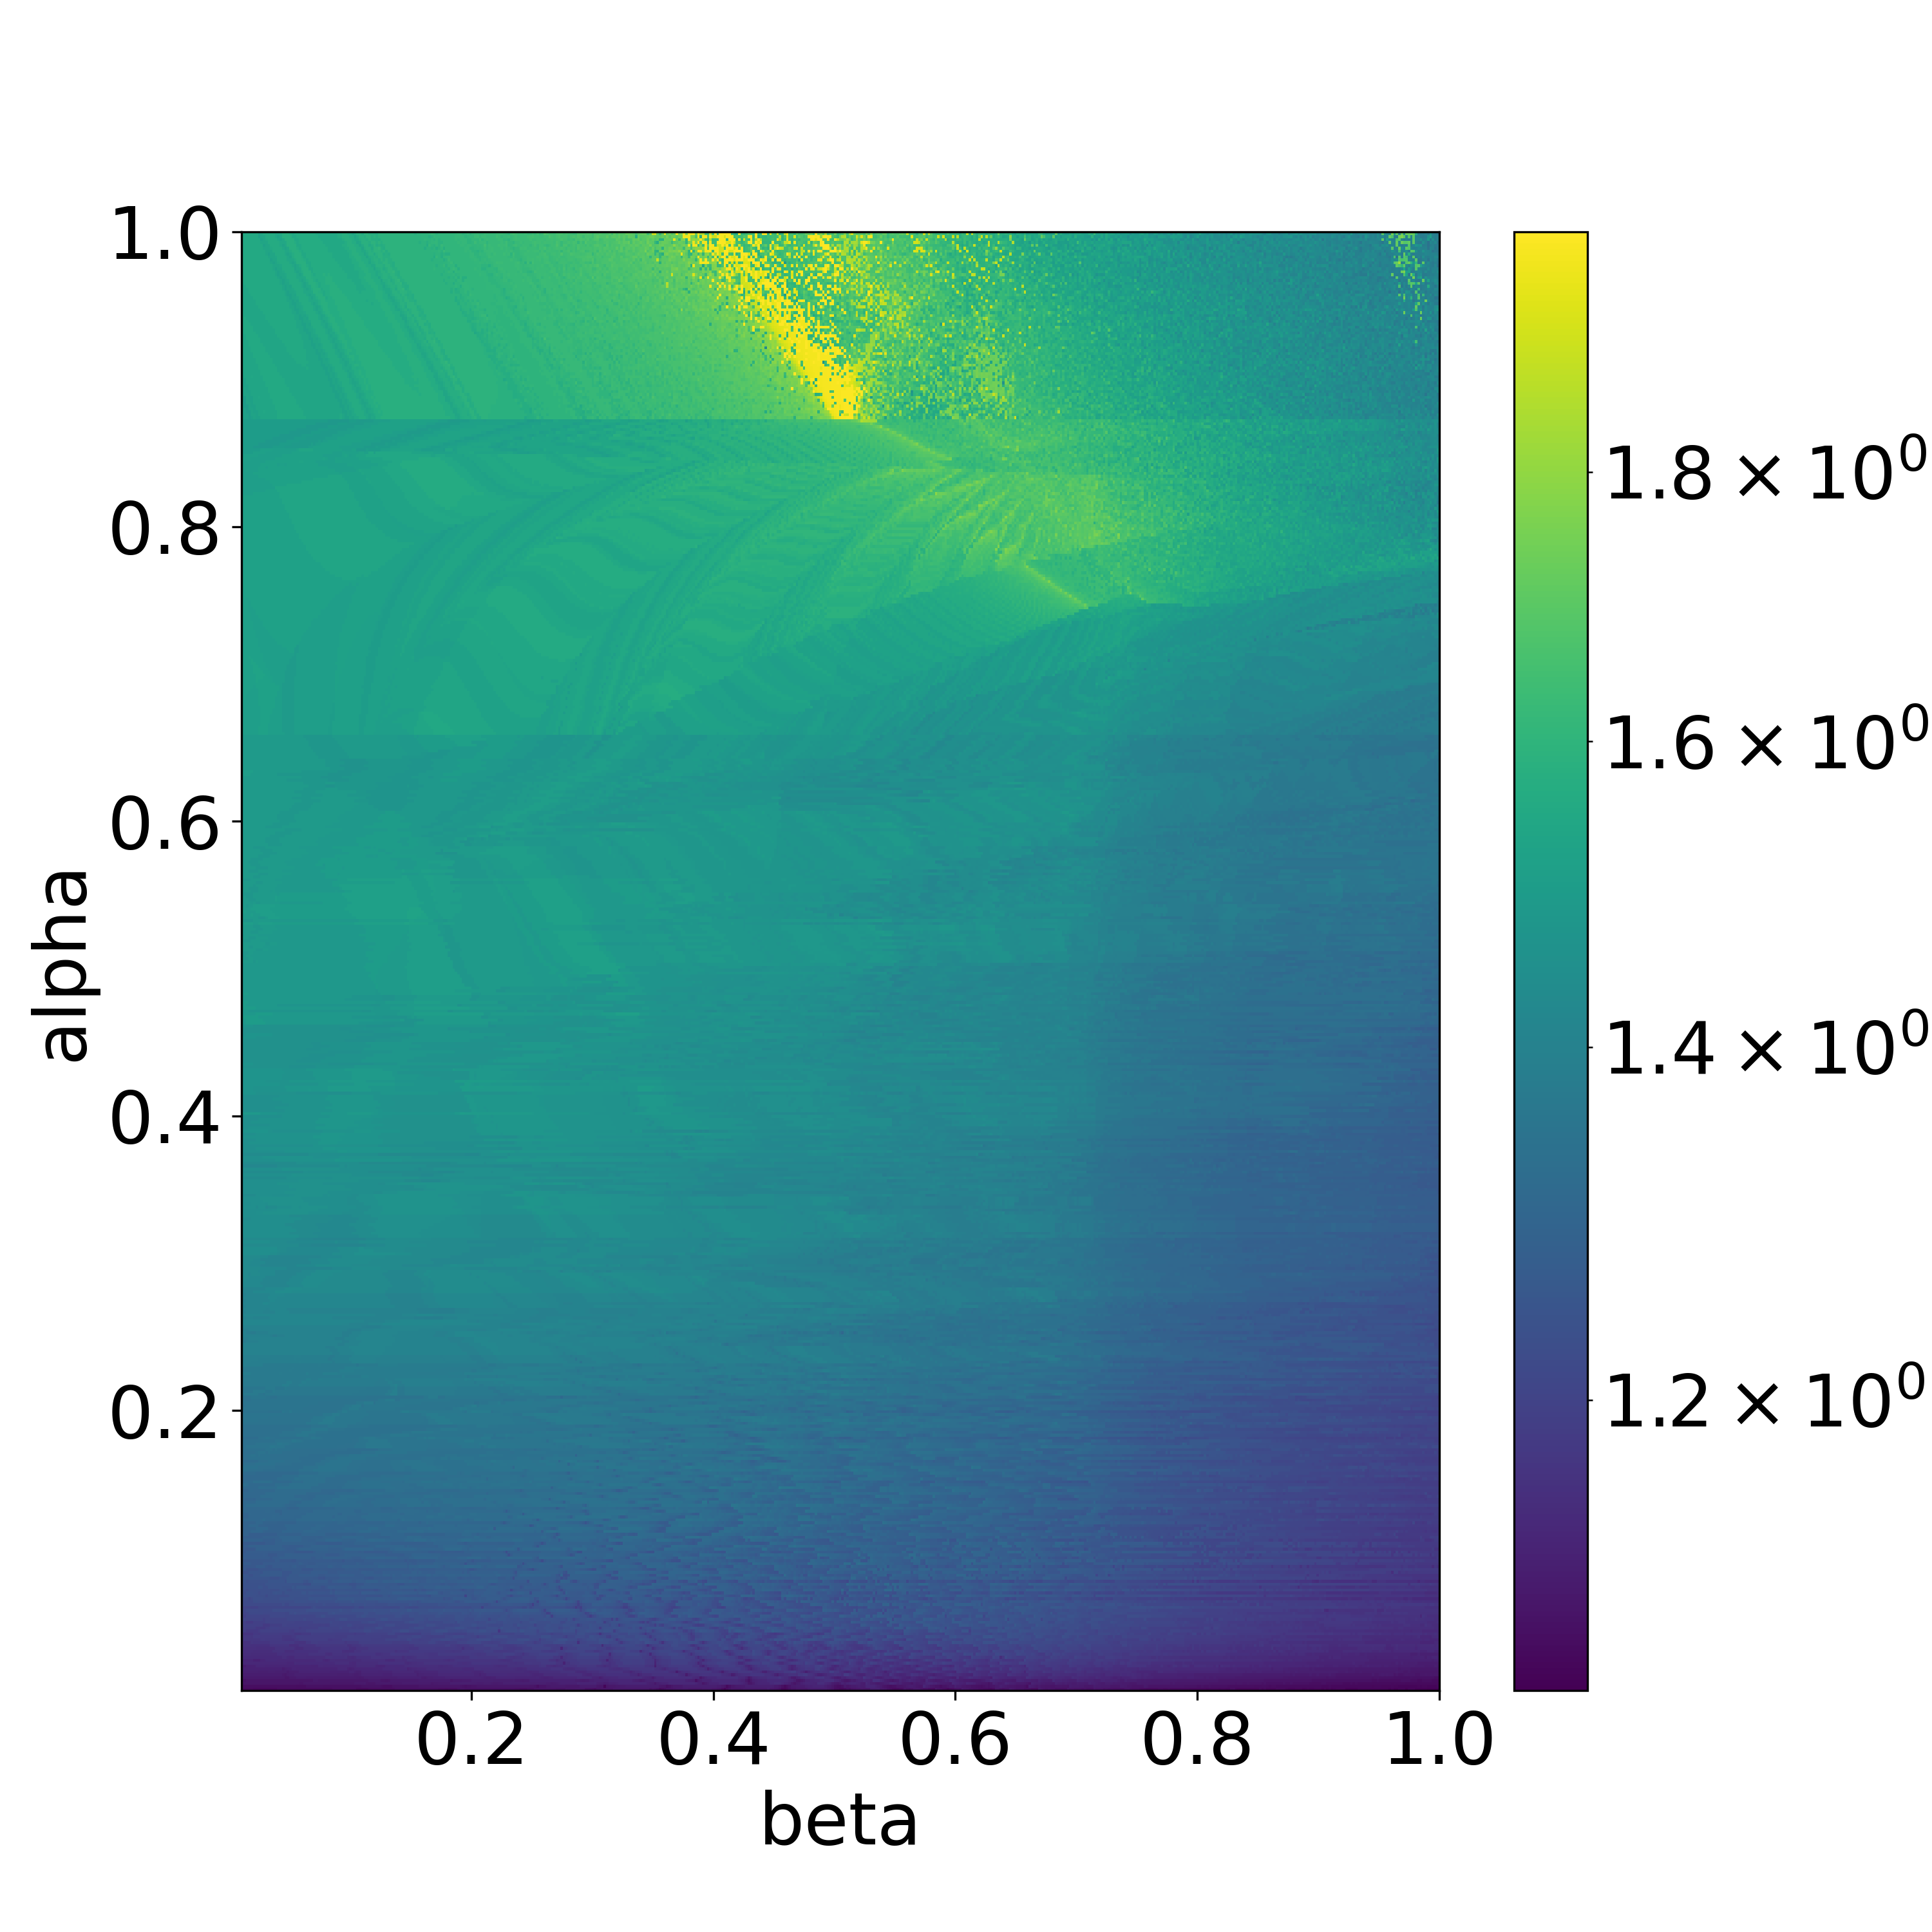
\includegraphics[width=1\textwidth]{images/analysis_BDF23_NI.png}
       	\subcaption{Average number of iterations per timestep} 
        \label{fig:numberIterationTSBDF23}
    \end{subfigure}
    \begin{subfigure}{0.32\textwidth}
    	\centering
    	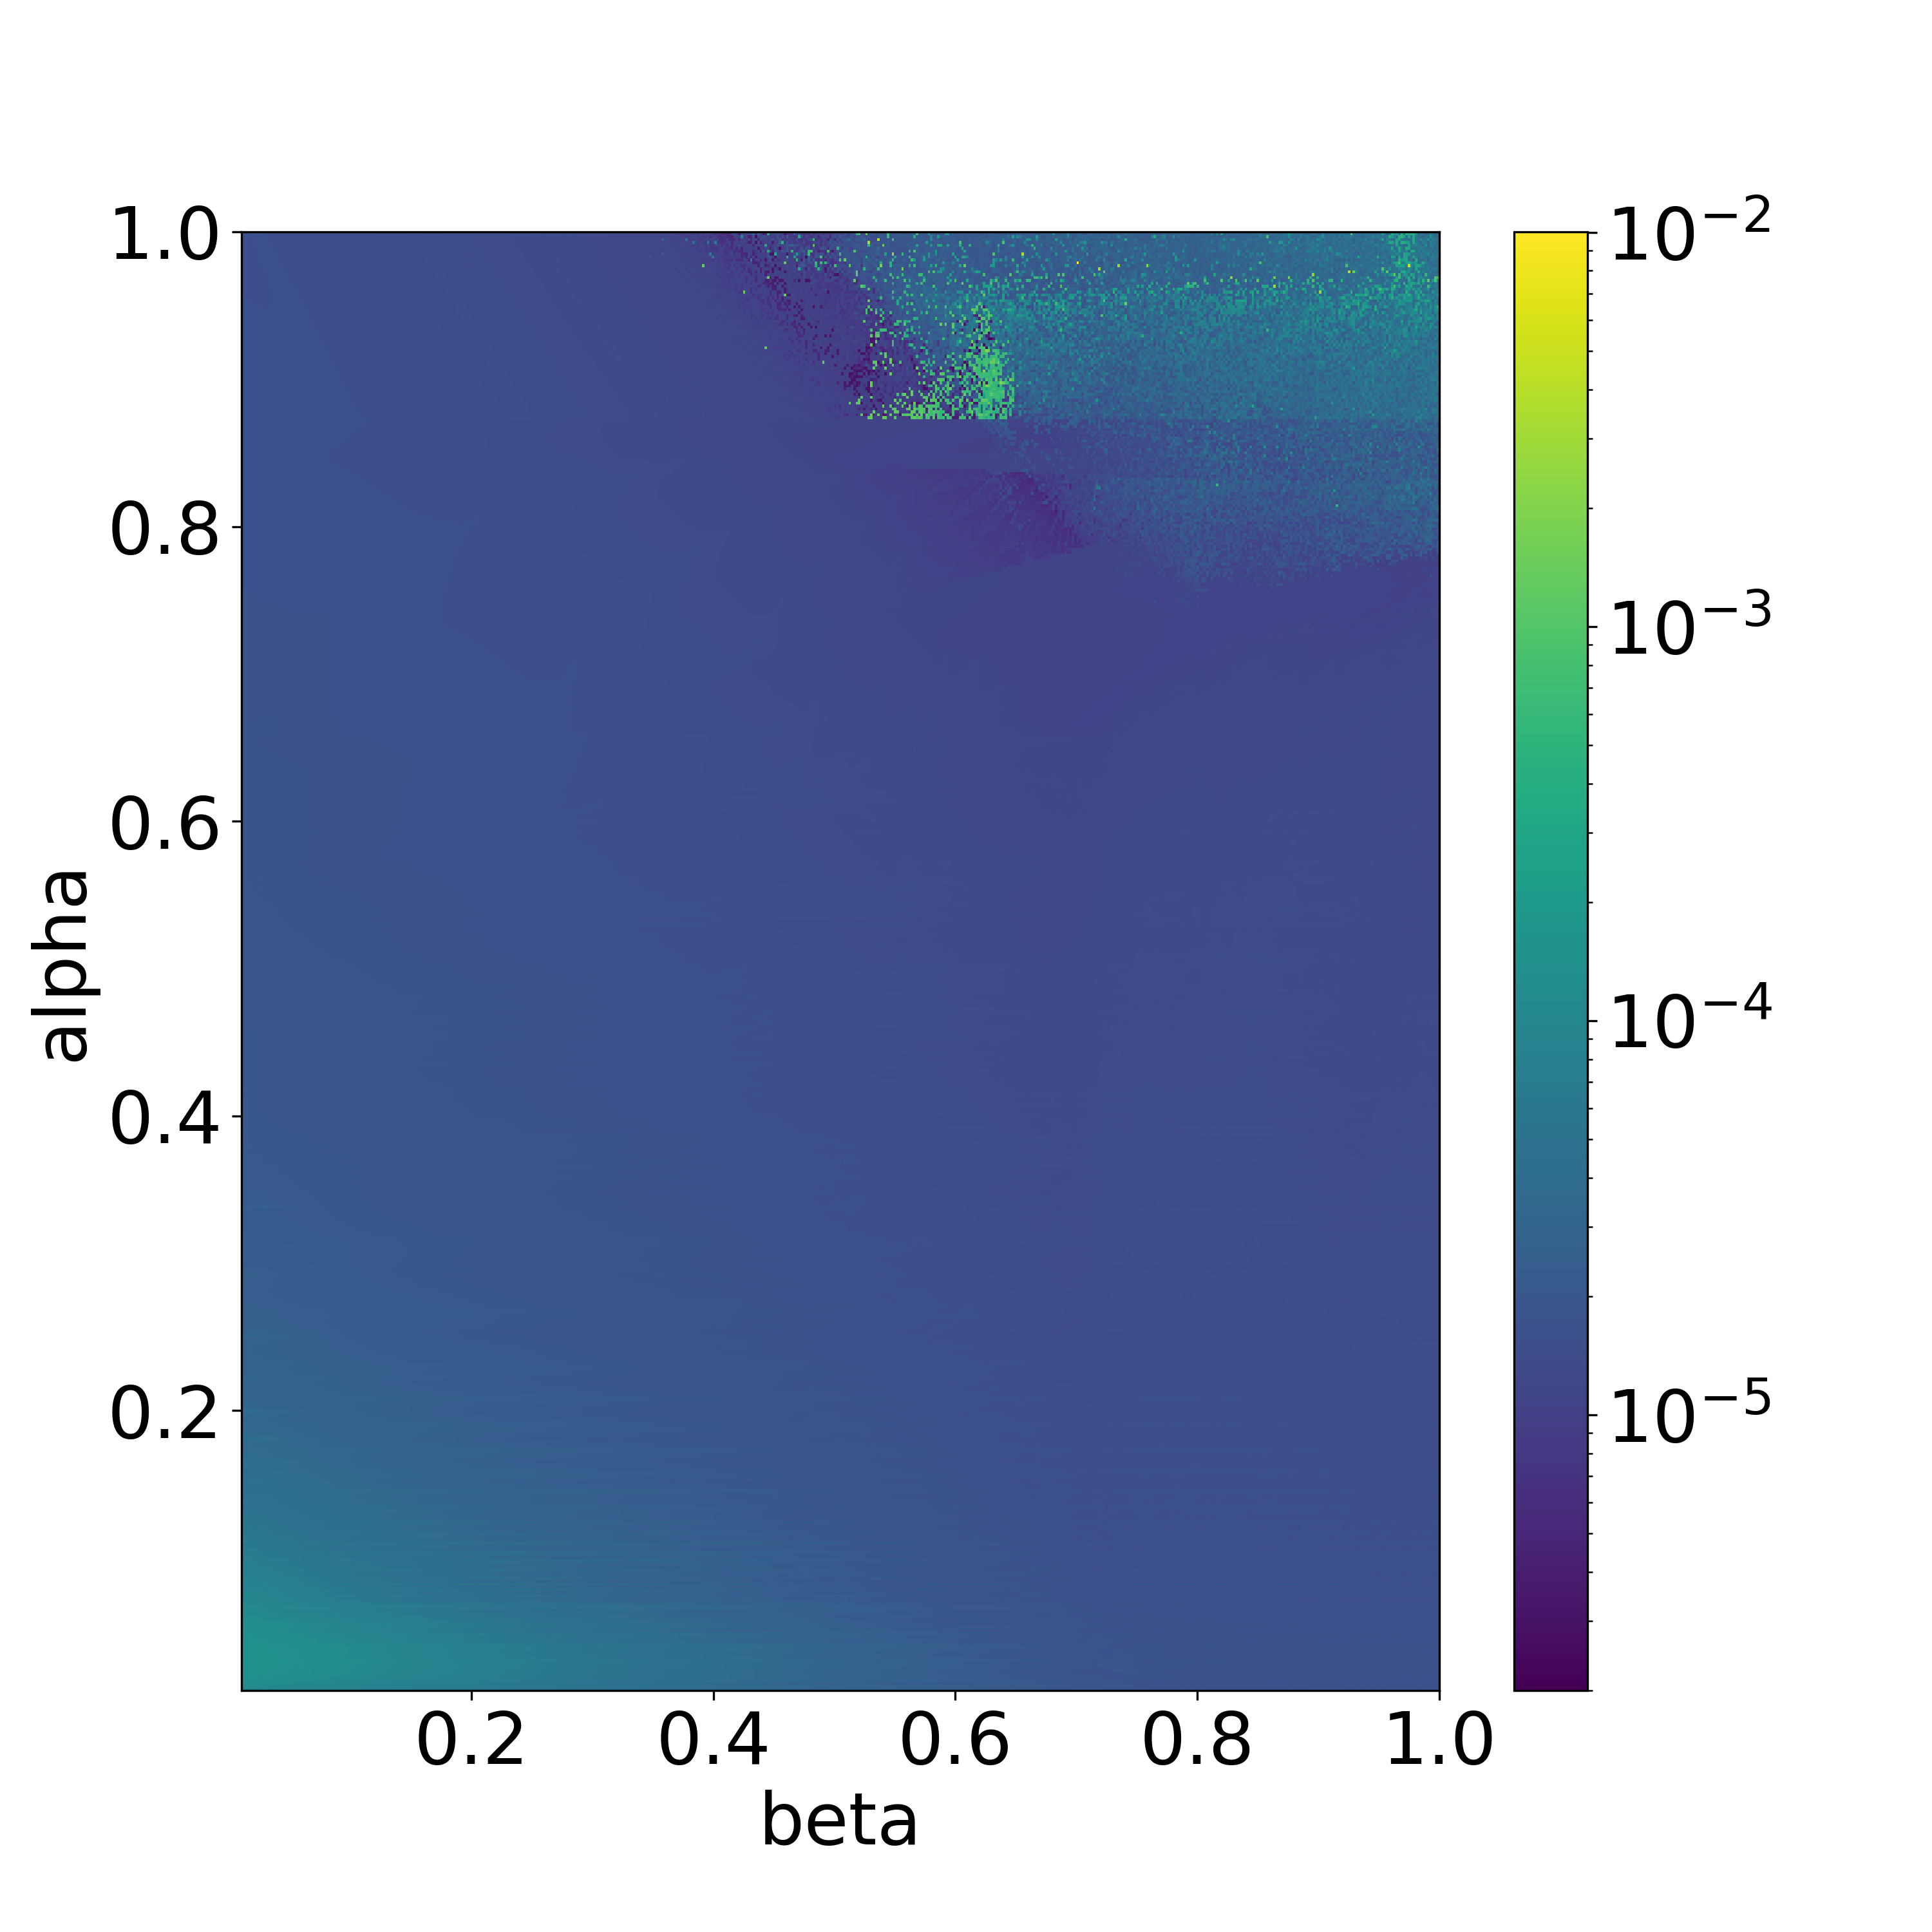
\includegraphics[width=1\textwidth]{images/analysis_BDF23_psi.png}
       	\subcaption{Absolute error of the variable $\psi$} 
        \label{fig:numberNumericalSchemeBDF23}
    \end{subfigure}
    \caption{Impact of the parameters $\alpha$ and $\beta$ of the PI controller on the number of required iterations to solve the model problem from \autoref{eq:first_DAE_ODE} using the implicit BDF method of second order (\textbf{BDF23}) for a simulation time of $t=5.0s$}
    \label{fig:ParametersPIControllerBDF23}
\end{figure}

We chose as parameters: 
\begin{itemize}
    \item for \textbf{RKF45}: $\alpha=0.4$ and $\beta=0.6$
    \item for \textbf{BDF12}: $\alpha=0.9$ and $\beta=0.4$
    \item for \textbf{BDF23}: $\alpha=0.9$ and $\beta=0.4$
\end{itemize}

---Put some more explanations here --- \\
---Find the balance between number of iterations and accuracy --- \\
---Numerical instabilities for the implicit methods for high values of $\alpha$ and $\beta$ --- \\
failure of the error estimate? too small timesteps? \\ 

\section{Comparison of the Numerical Schemes}
So far, one explicit (RKF45) and two implicit (BDF12, BDF23) numerical solvers have been implemented for the initial DAE in \autoref{eq:first_DAE_algeb} and their ideal parameter choice for their use with a PI controller has been discussed. Now, the quality of the solutions is compared. \\
Again, the allowed tolerance of the PI controller is set to $\epsilon=1\cdot 10^{-6}$. The method of the manufactured solutions is chosen to have an analytical solution against which numerical computations can be compared. The parameters $t_e$ and $t_w$ are chosen in a way that the velocity is initially close to zero and increases to 1 over the time span of one second at the middle of the simulation time. \autoref{fig:timeEvolutionValues} depicts the solution variables $\psi$ and $V$ over time for all three solvers. The expected form of the $\text{atan}$ function centered around $2.5$ for the velocity is obtained with all methods and the results for $\psi$ match too, as $\psi$ decreases linearly before it stabilizes around zero as the velocity increases. \\
If adaptive timestepping methods are used, the actual size of the timestep $h_n$ is of particular interest. Since at each timestep, the right-hand side of the ODE and the algebraic equation have to be solved a fixed number of times, a method that allows larger timesteps is considered more efficient. As shown in \autoref{fig:timeEvolutionDT}, this metric varies greatly with the chosen numerical solver. The simulation time can be roughly split into three sections: The first phase corresponds to low velocity and decreasing $\psi$ until the time $t=2.0s$. In it, the RKF45 and BDF23 methods allow for rather similarly large timestep sizes, whereas the BDF12 method is restricted to timestep sizes which are about fives times smaller. The second phase is marked by the fast increase in velocity and the stabilization of $\psi$. Such rapid changes in the solution should imply shorter timesteps to obtain accurate solutions, especially for RKF45, because explicit schemes face stability issues for stiff problems. Indeed, a decrease in the timestep size can be observed for all three methods, however the explicit RKF45 performs much better than expected with timesteps that are about twice as long as using BDF23. As previously, BDF12 has the worst performance of all three methods which much smaller timesteps. In the last phase, when the velocity approaches 1 and $\psi$ remains close to 0, the two implicit BDF methods reach very large timesteps with an increasing trend, whereas the the timesteps generated by the controller RKF45 stagnate at a rather low value. Overall, BDF23 performs best with 69 timesteps, followed by RKF45 with 120 and finally BDF12 needs 230 timesteps to execute the whole simulation. 

\begin{figure}[H]
    \centering
    \begin{subfigure}{0.43\textwidth}
    	\centering
    	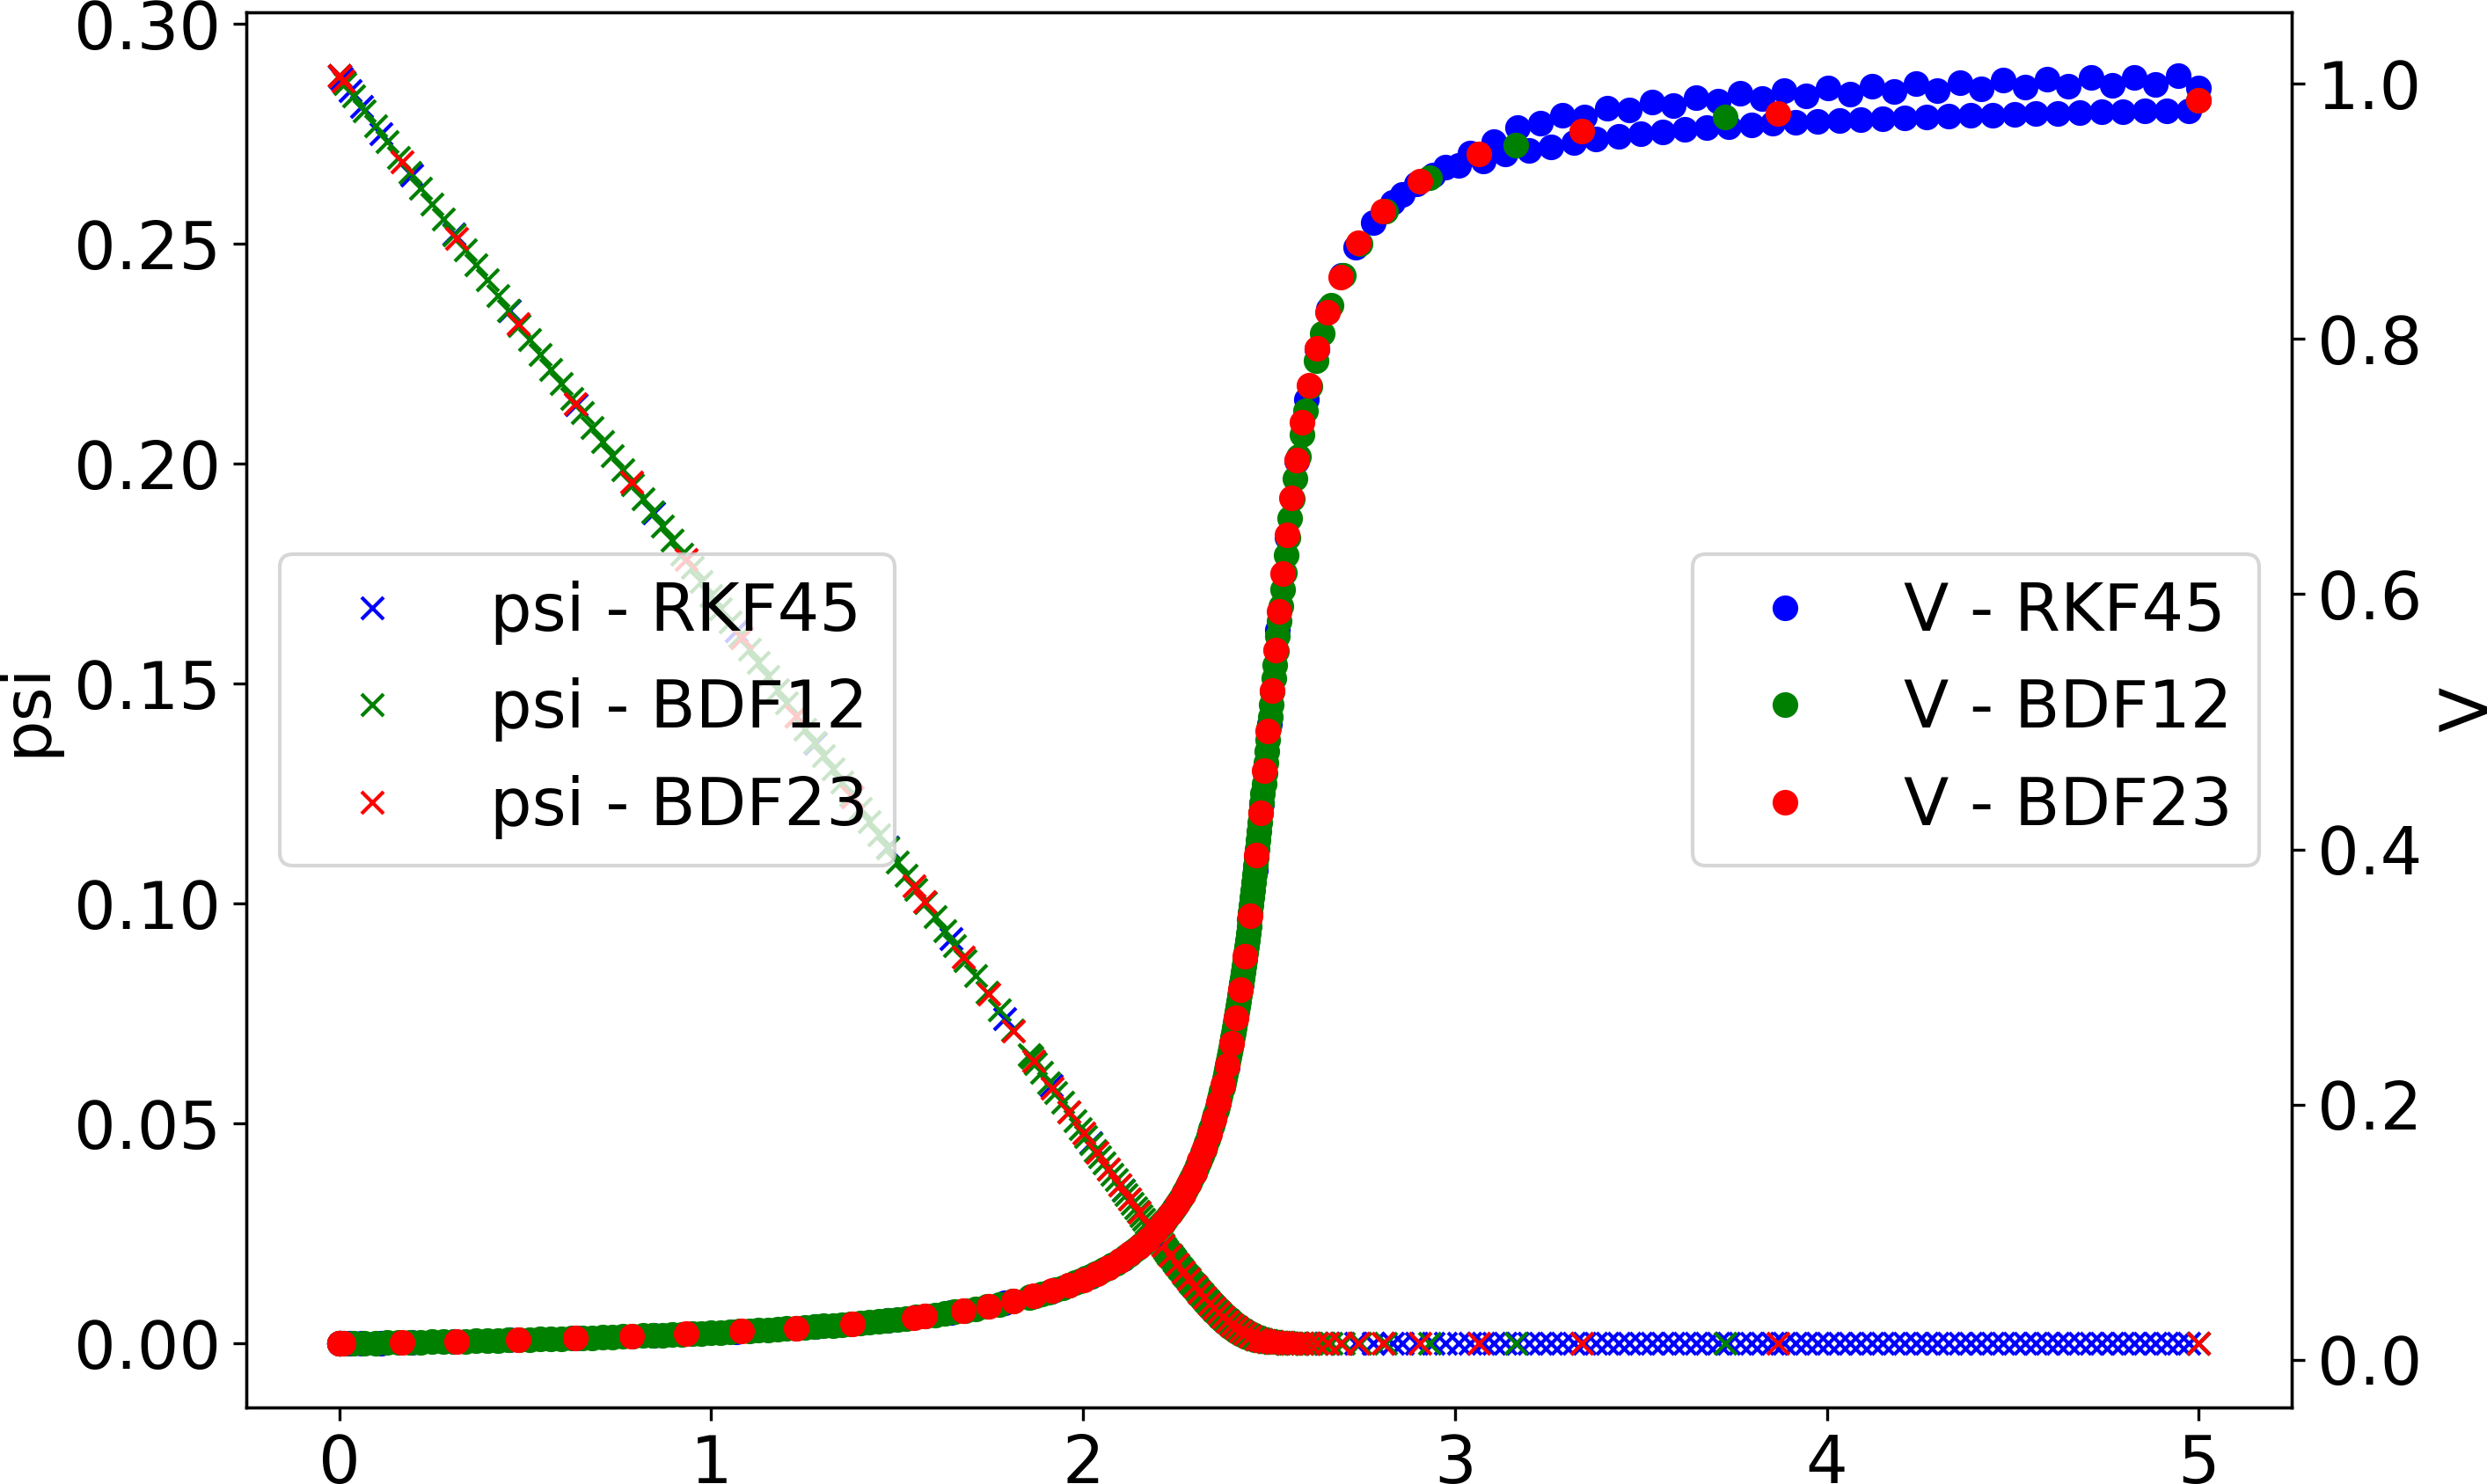
\includegraphics[width=1\textwidth]{images/timeEvolutionValues.png}
       	\subcaption{Evolution of the velocity $V$ and of the state variable $\psi$} 
        \label{fig:timeEvolutionValues}
    \end{subfigure}
    \begin{subfigure}{0.43\textwidth}
    	\centering
    	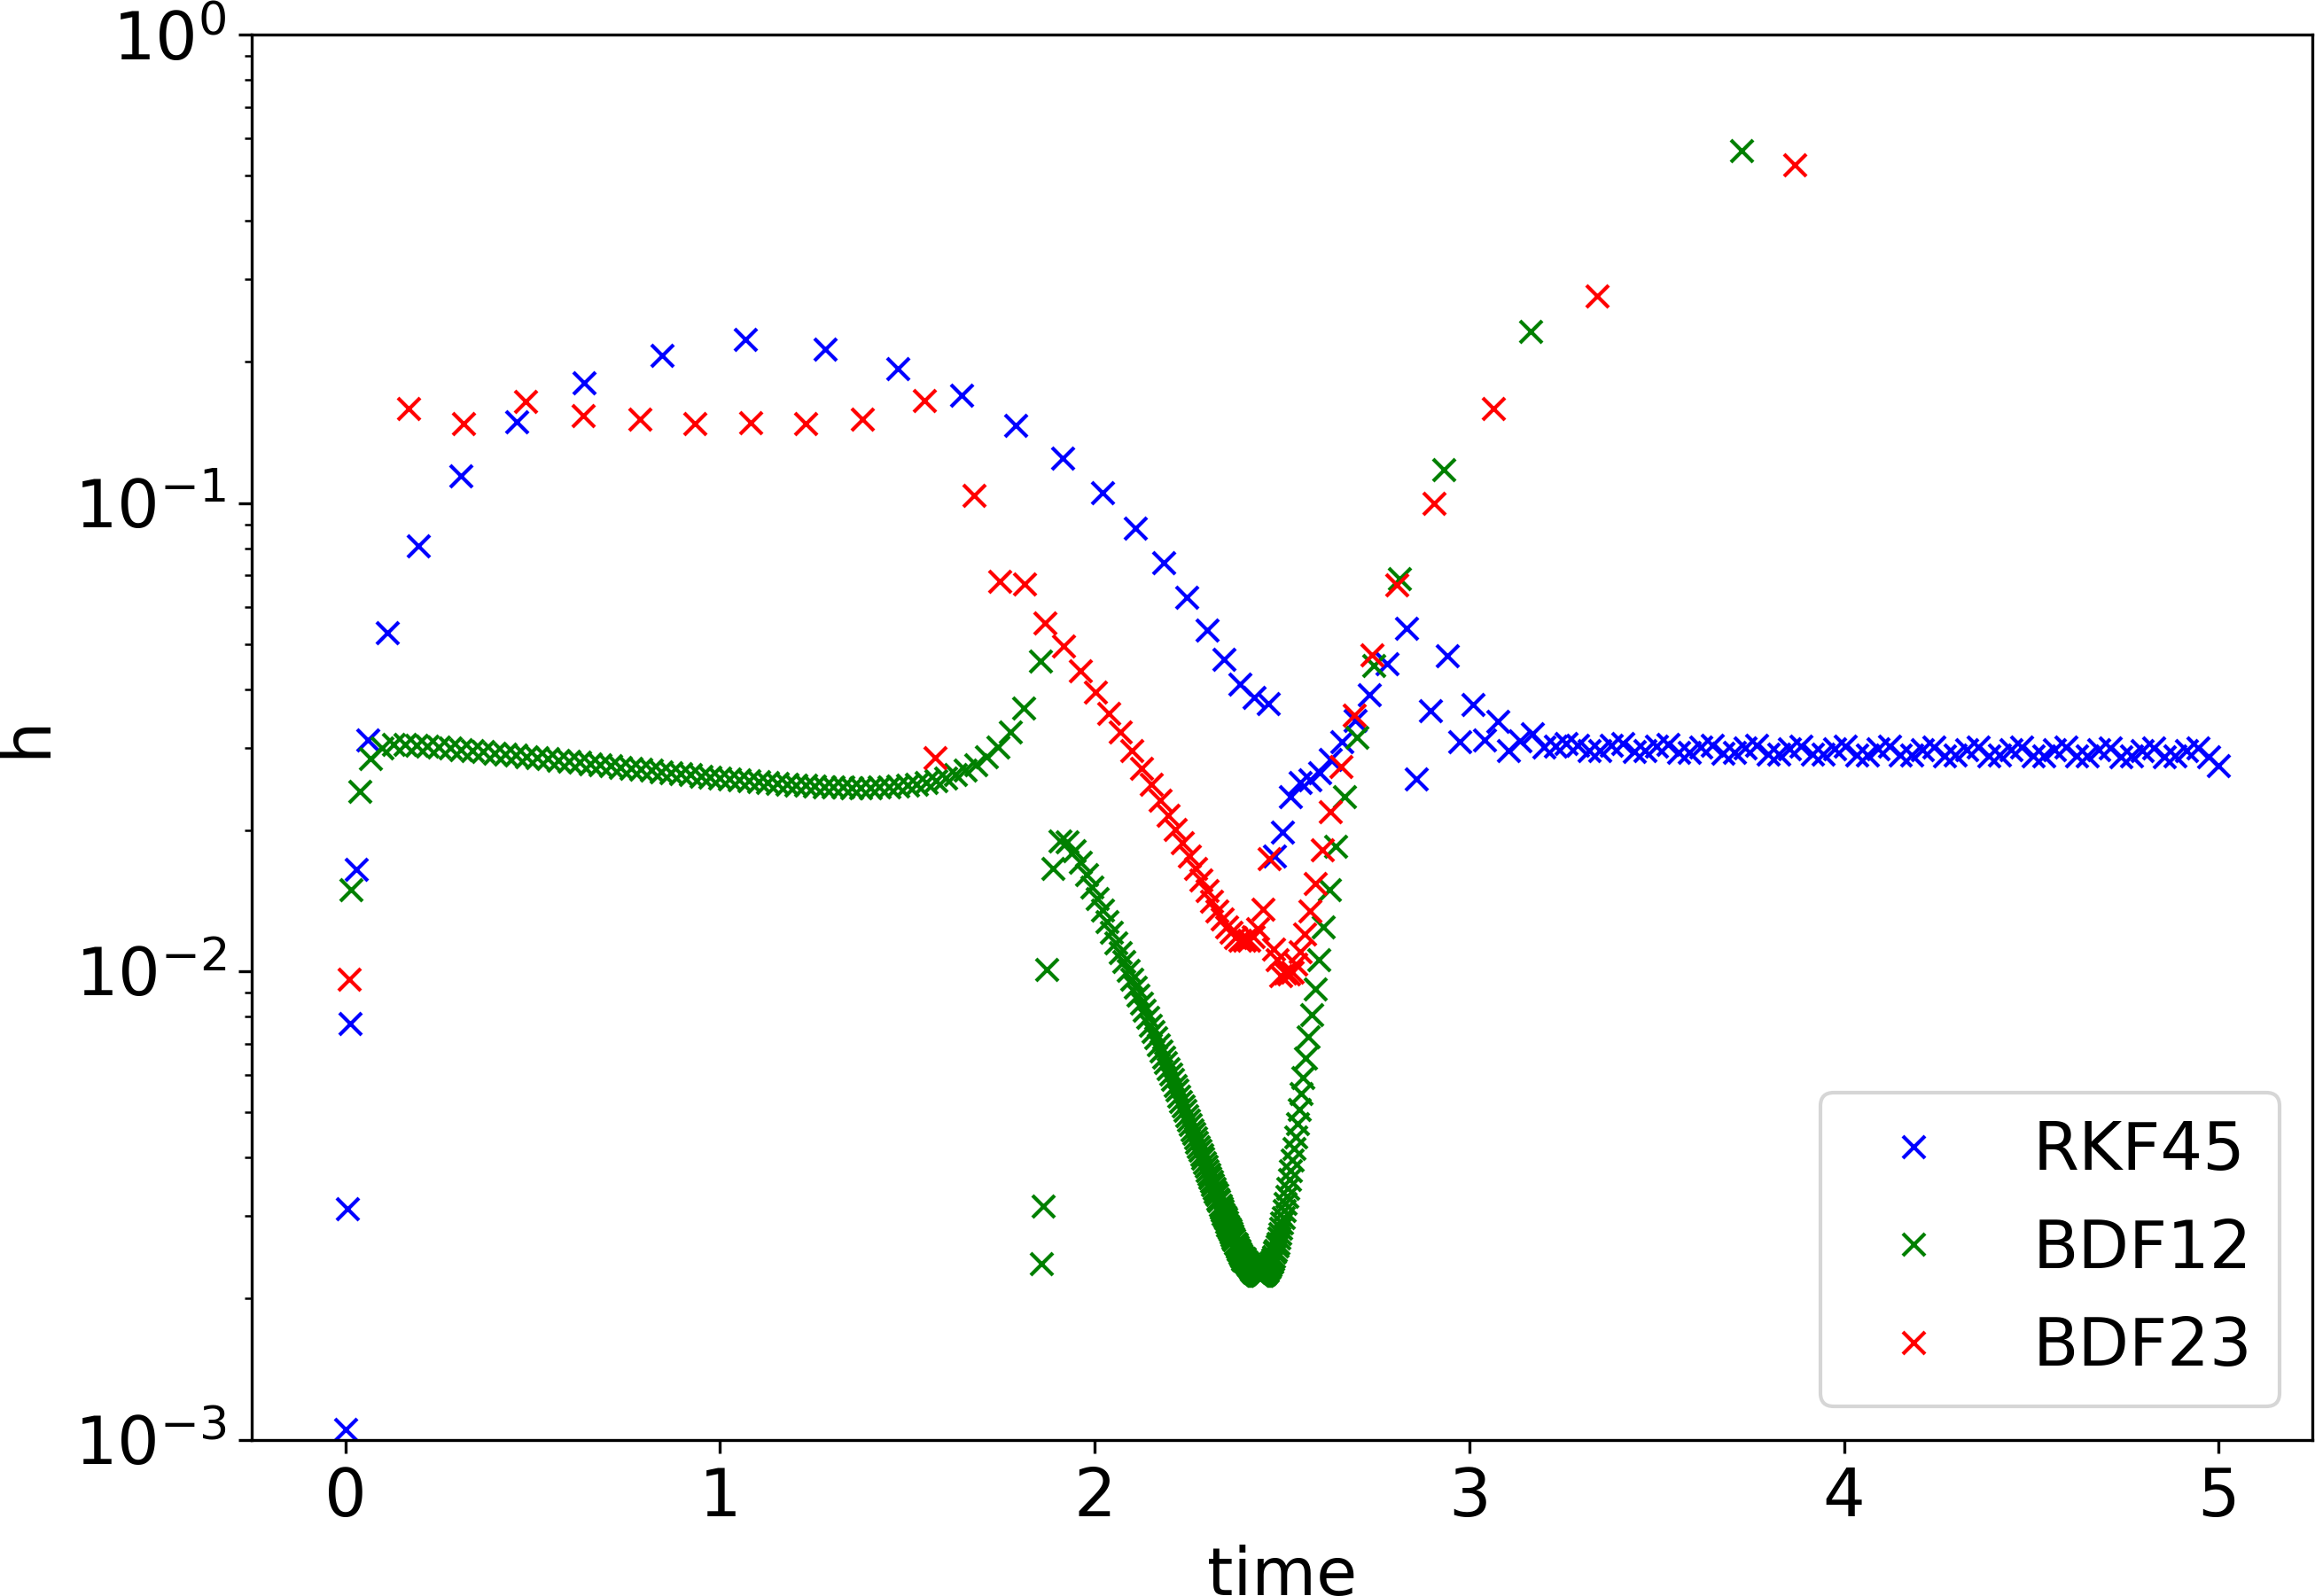
\includegraphics[width=1\textwidth]{images/timeEvolutionDT.png}
       	\subcaption{Evolution of the timestep size $h_n$} 
        \label{fig:timeEvolutionDT}
    \end{subfigure}
    \caption{Evolution of the solution and the timestep sizes of the single state problem defined in \autoref{eq:first_DAE_algeb} with the implemented numerical schemes}
\end{figure}

Now, the accuracy of the three numerical methods is compared. Therefore, \autoref{fig:timeEvolutionErrorPSI} depicts the evolution of the absolute difference between the numerical solution and the analytical solution of the state variable $\psi$. It is of interest to compare this error with the absolute error in velocity, shown in \autoref{fig:timeEvolutionVerror}. \\ 
As $\psi$ decreases, the error in $\psi$ increases steadily for all three numerical solvers. The implicit BDF methods produce two peaks in the evolution of the error, the first shortly before the end of the decrease and the second at the stiff transition of the velocity from 0 to 1. The norm of the error is much higher for BDF12 than for BDF23, despite the lower number of timesteps of the latter. The explicit RKF45 method produces a similar error norm as BDF12, but only in one peak at the beginning of the transition phase. In the end of the simulation, when $\psi$ stays around 0, all solvers match closely with the analytical solution and the error remains very low. On the other hand, the error in the velocity is very low for all solvers at the beginning and a peak in the error appears at the transition from 0 to 1. As usual, the highest error here appears for BDF12. Between the two remaining methods, RKF45 has the lowest error, which is astonishing for an explicit method applied to a stiff problem, especially considering the fact that in this section of the simulations, it also allows larger timesteps. Towards the end of the simulation, the error in velocity obtained by the two implicit methods vanishes again, however RKF45 produces suddenly very high errors which alternate between three different values. In \autoref{fig:timeEvolutionValues}, it can be seen that the velocity oscillates around the expected solution without getting closer to it. \\
It is important to realise that the error in $\psi$ and in the velocity are not directly correlated, thus a small error in $\psi$ does not necessarily lead to a small error in the velocity. It might thus be wise to reconsider the way the timestep size is controlled. So far, it only depends on the ratio between the local truncation error and a predefined tolerance value. This error is estimated by applying another numerical scheme with higher order, by taking the difference in $\psi$ of the two solutions as error estimate. Therefore, the velocity is not involved in the step size controller and the controller cannot ensure that the chosen timestep size guarantees sufficiently accurate results for the velocity. To ensure correct physical results, the controller needs to be extended in a way to restrict the timestep size with respect to some error estimate of the velocity. 

\begin{figure}[H]
    \centering
    \begin{subfigure}{0.43\textwidth}
    	\centering
    	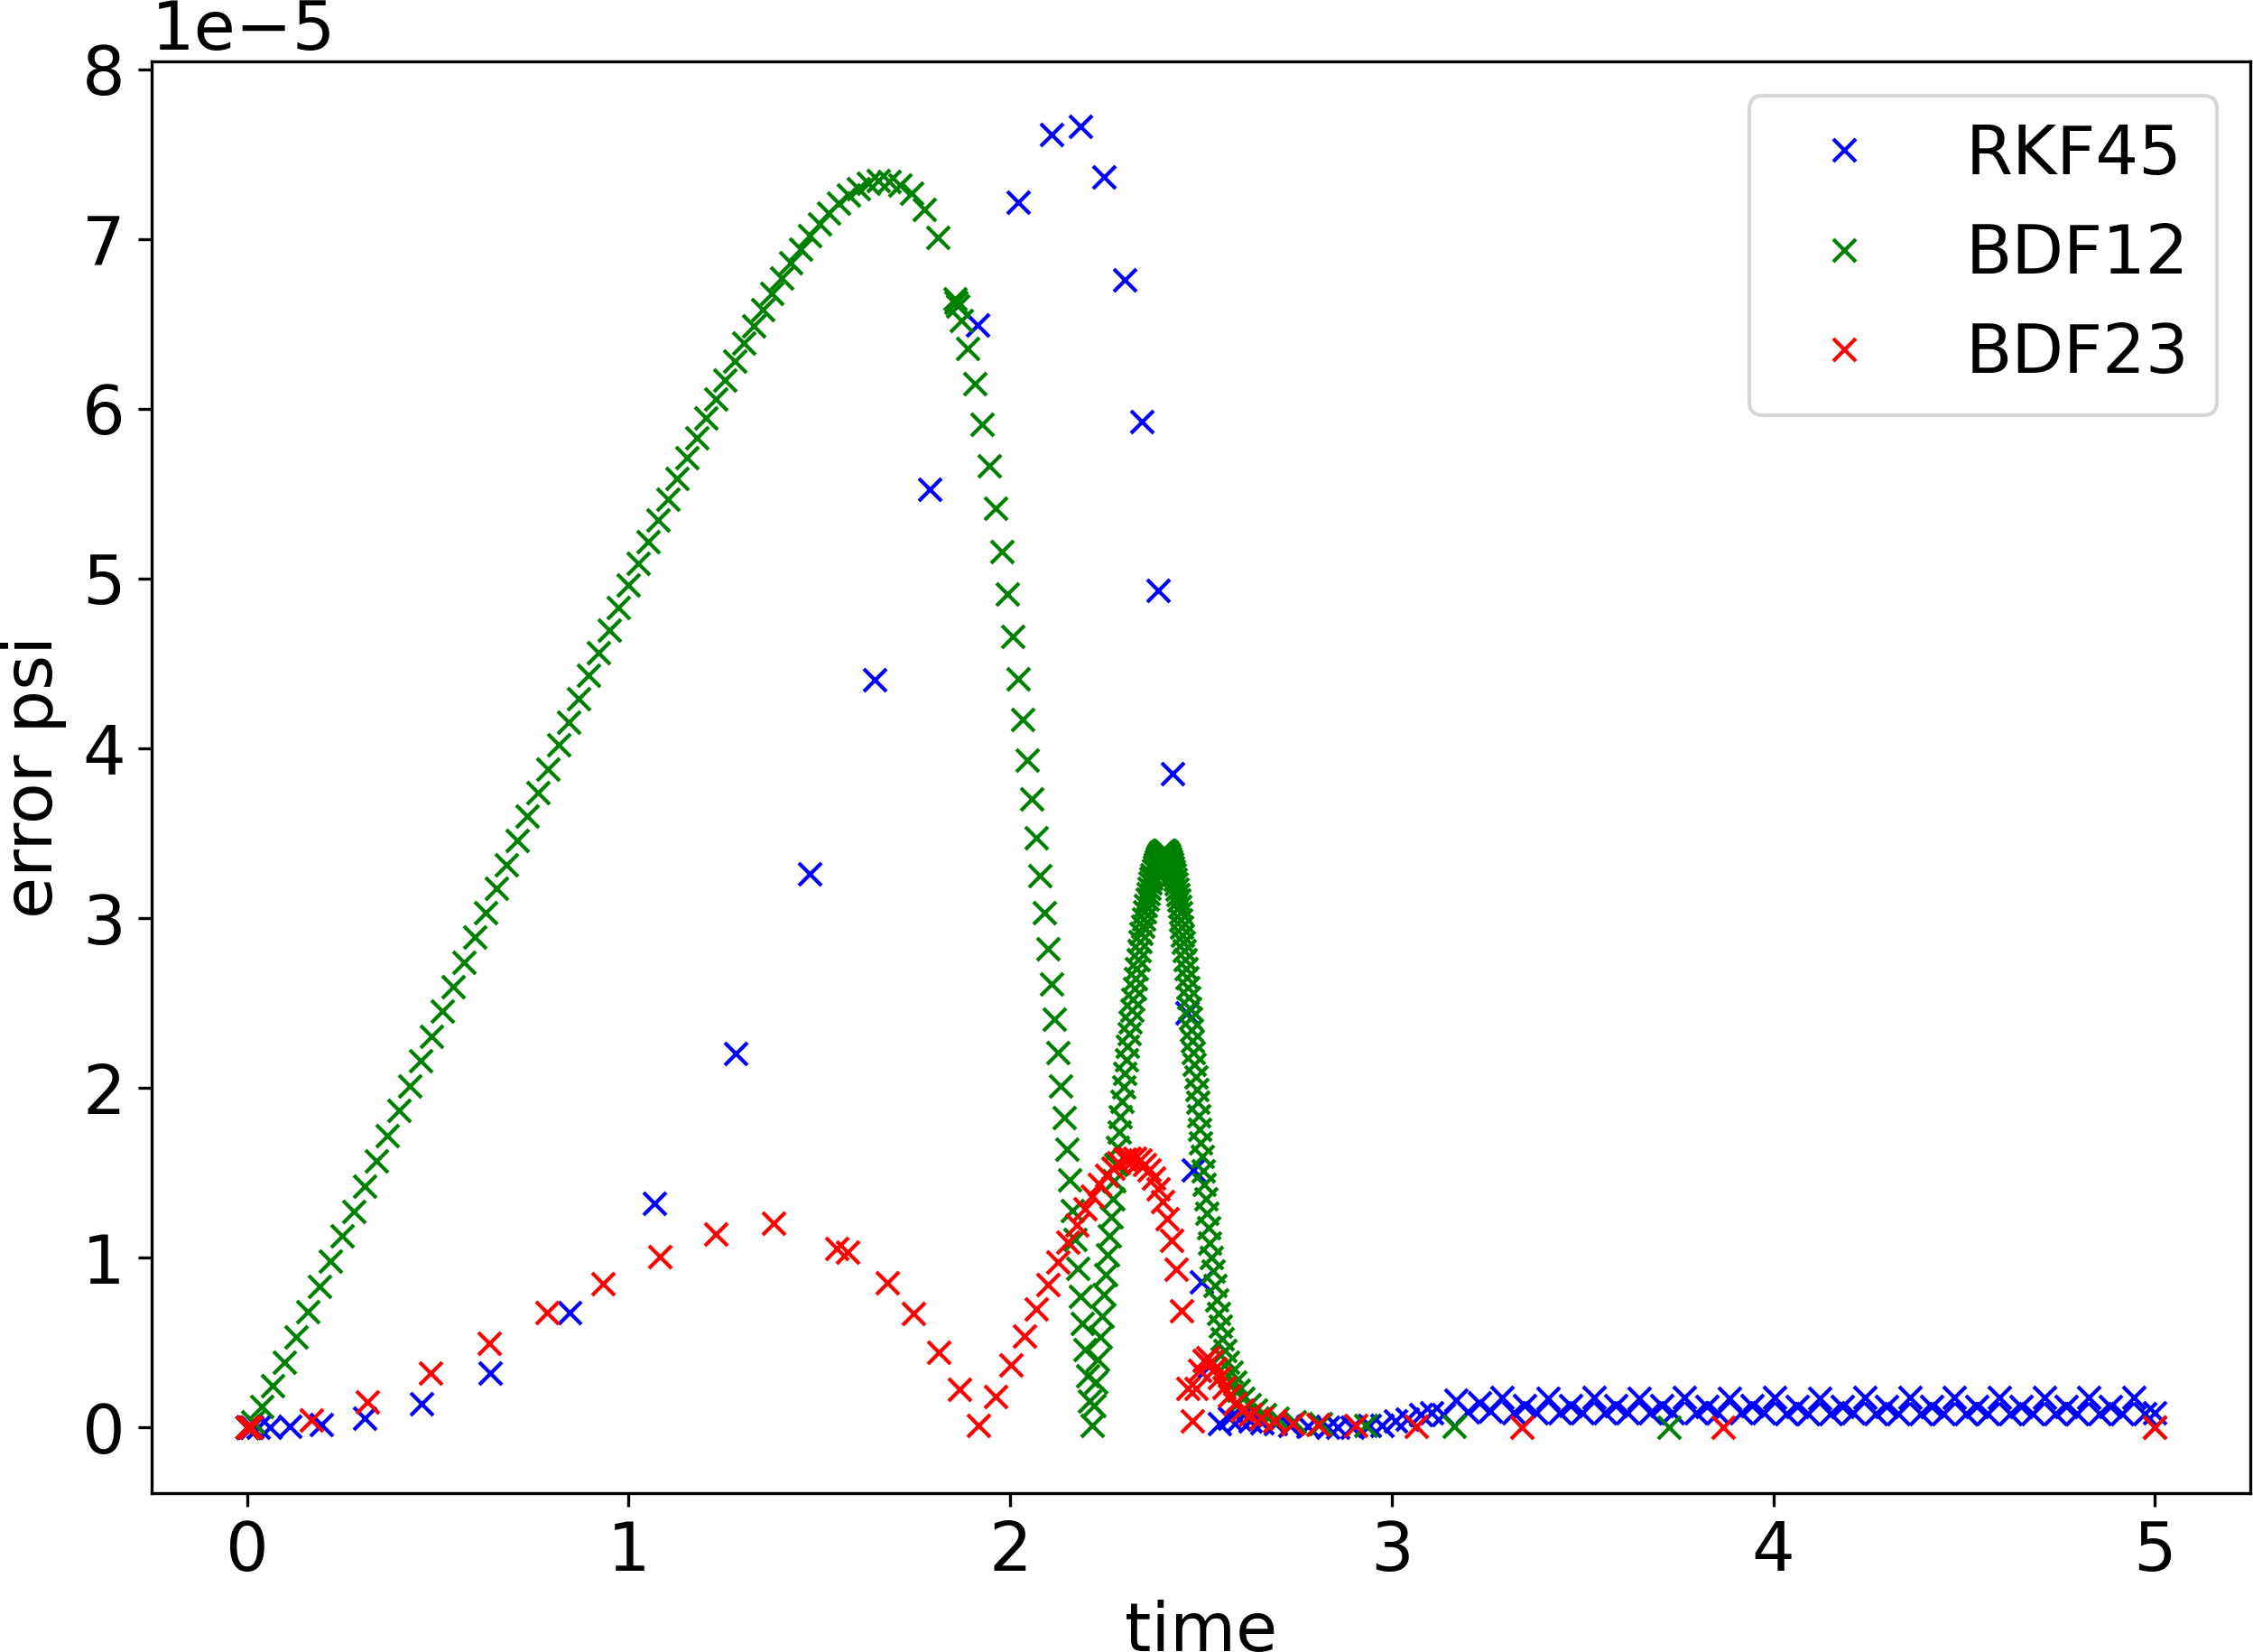
\includegraphics[width=1\textwidth]{images/timeEvolutionPSIerror.png}
       	\subcaption{Evolution of the absolute error of the state variable $\psi$} 
        \label{fig:timeEvolutionErrorPSI}
    \end{subfigure}
    \begin{subfigure}{0.43\textwidth}
    	\centering
    	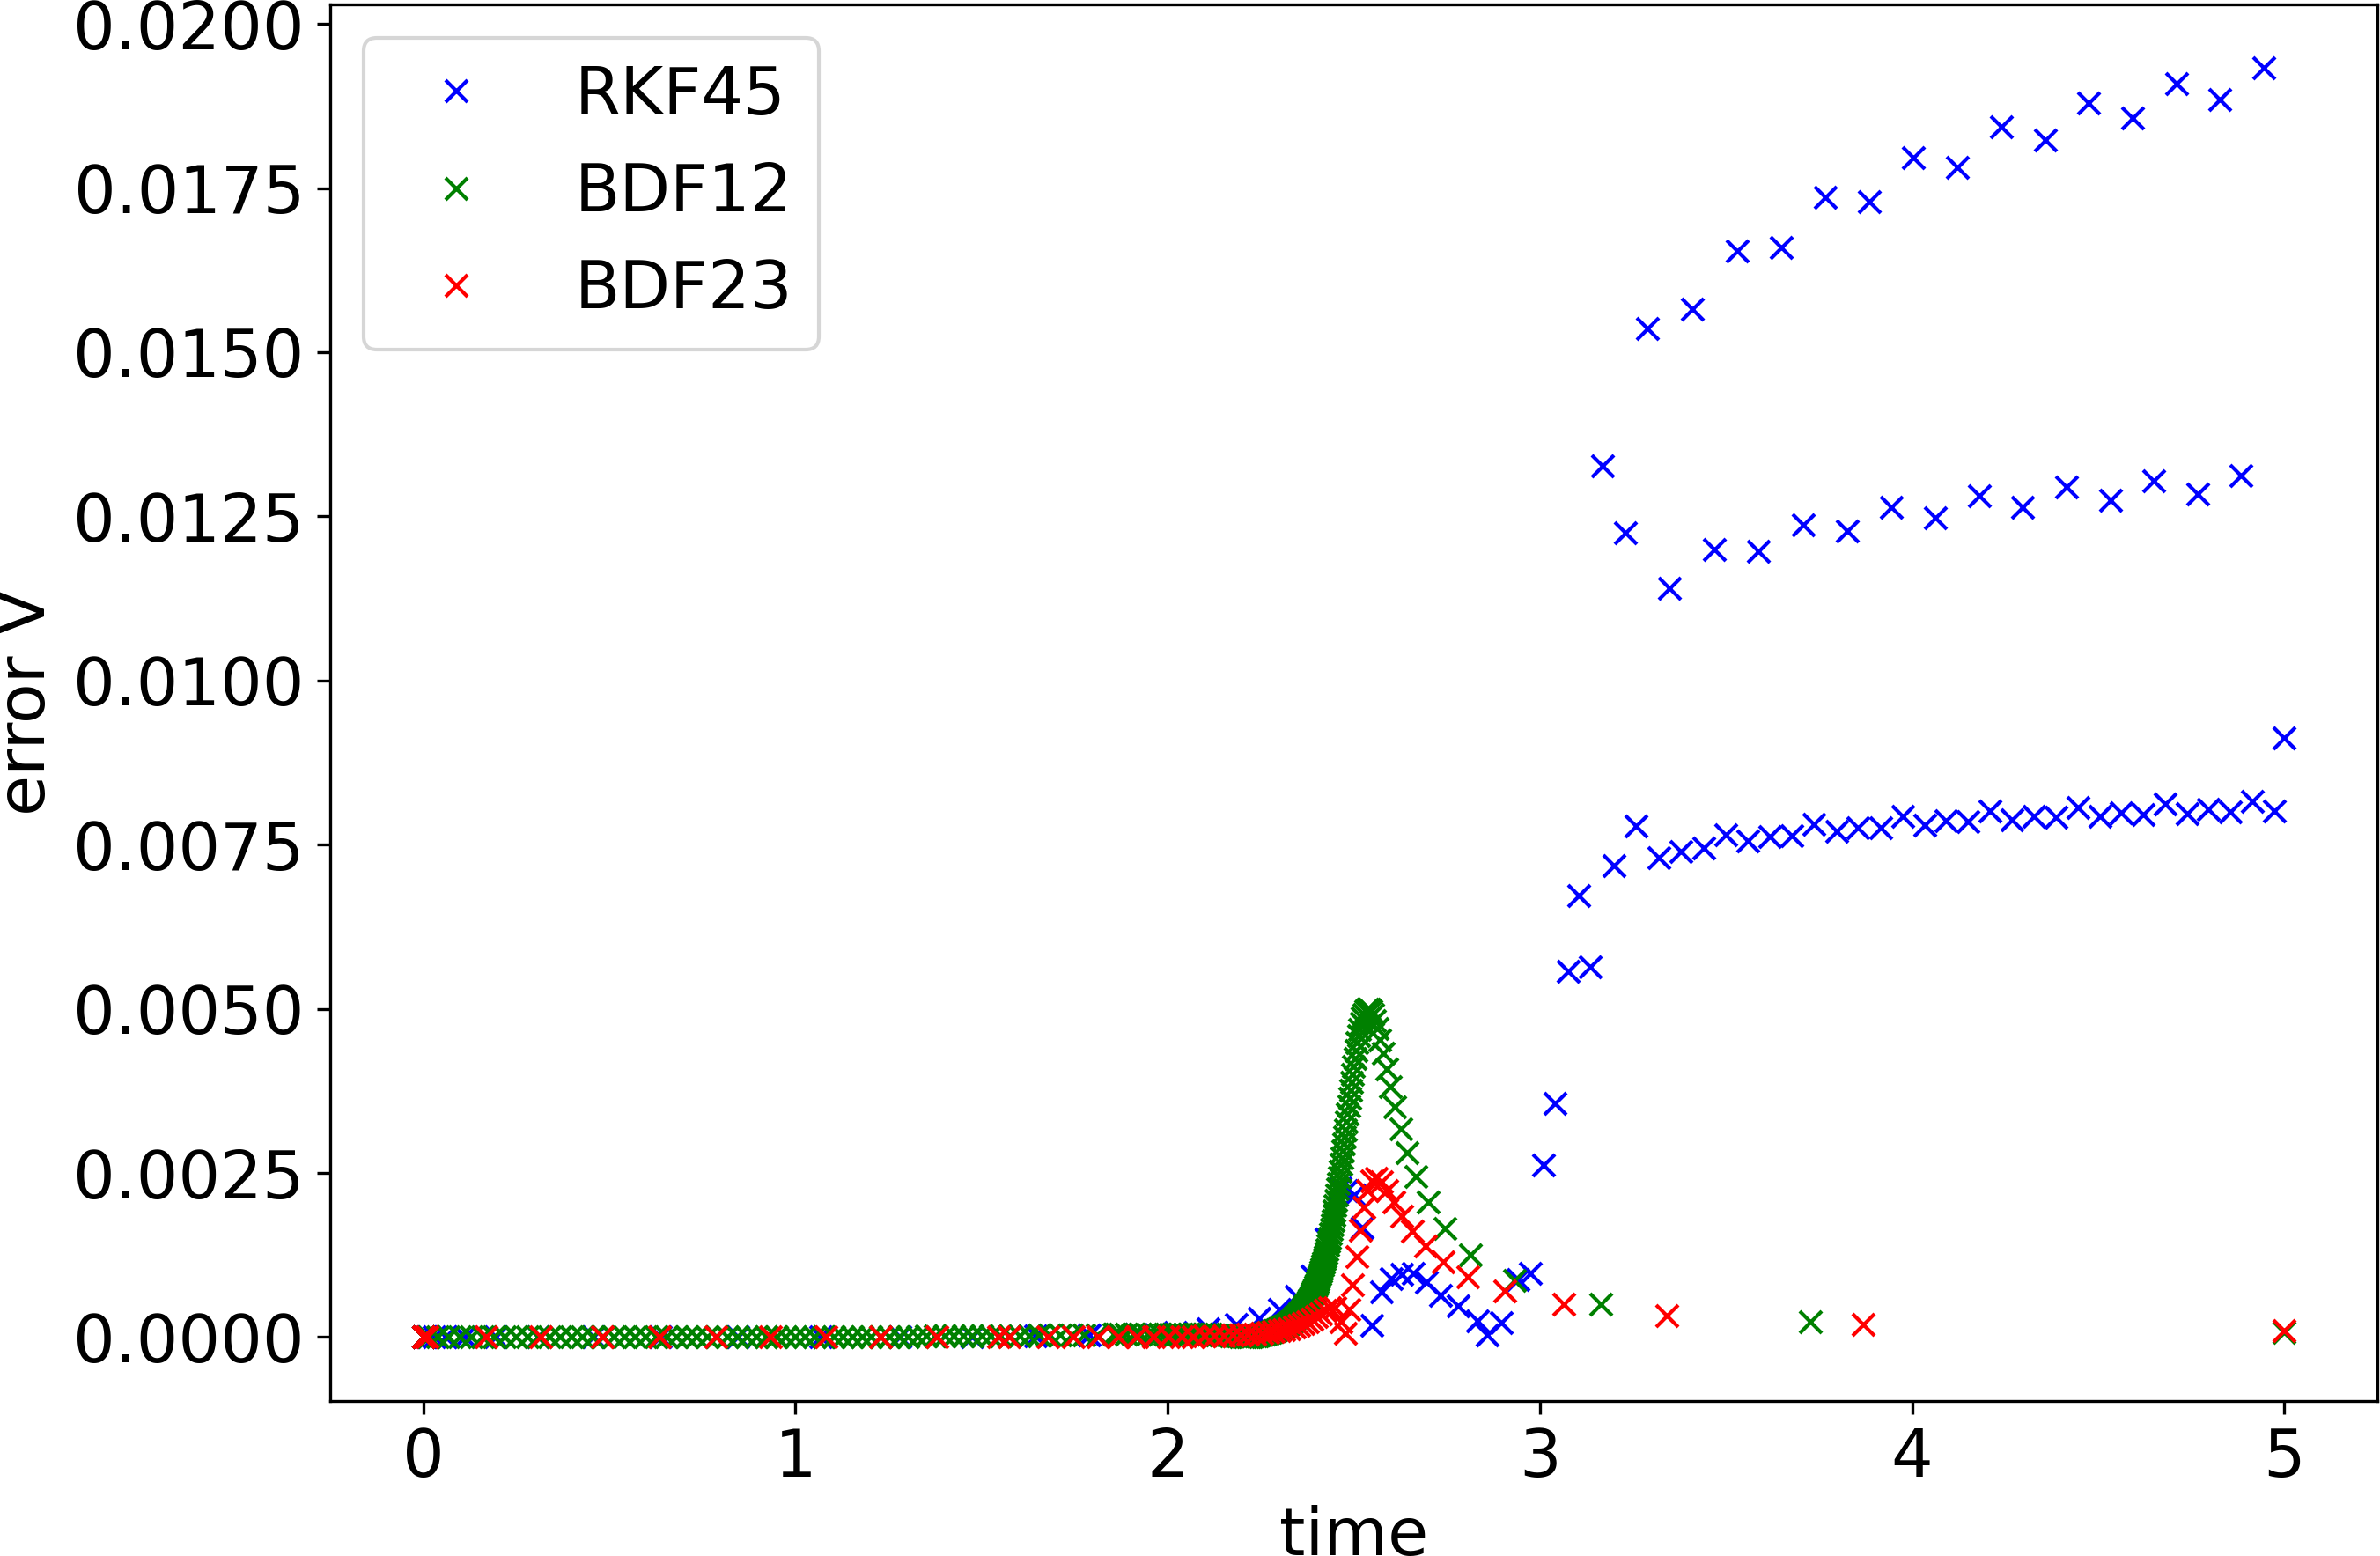
\includegraphics[width=1\textwidth]{images/timeEvolutionVerror.png}
       	\subcaption{Evolution of the absolute error of the velocity $V$} 
        \label{fig:timeEvolutionVerror}
    \end{subfigure}
    \caption{Evolution of the error for the single state problem defined in \autoref{eq:first_DAE_algeb} with the implemented numerical schemes}
\end{figure}

The whole theory of PI controller bases on an accurate error estimate, which is obtained in our case by calculating the solution with a higher order method. It is interesting to analyze whether the error estimate calculated in this way matches with the actual error to the analytical solution. The absolute error cannot be used as in the previous graphs, since the error estimate is calculated from the lower-order solution at the previous timestep. On the other hand, the local truncation error, which measures by how much the total error increases at each timestep, is much better suited to evaluate the accuracy of the error estimate. \\
In \autoref{fig:errorEstimateEvolutionALL}, the difference between the two solutions calculated at each timestep by any of the schemes, being the error estimate, plotted against the real local truncation error. In the initial phase, the two implicit methods estimate the error very closely to its real value. Even though the BDF12 method approximates it better than the BDF23 method, the high amount of executed timesteps in this phase accumulate the total error which turns out to be much worse. The estimate of the explicit RKF45 method roughly follows the real evolution of the local truncation error, but underestimates it by a large factor up to 5. During the transition phase, the situation is reversed, because the implicit methods fail at estimating correctly peaks in the evolution of the real error and remain instead around a same value. On the other hand, the RKF45 follows much better the evolution of the local truncation error, which explains its good performance in the transition phase with respect to the allowed timestep size and to the total error. In the final phase, the two implicit methods match again with the expected error values and the RKF45 method seems to fit exactly the real error, but it shows nonphysical oscillations which seem to correspond to the larges oscillations in the total error of the velocity. \\
Overall, the implicit methods yield the better error estimates except for the stiff transition which seems to be better handled by the explicit scheme. 

\begin{figure}[H]
    \centering
    \begin{subfigure}{0.32\textwidth}
    	\centering
    	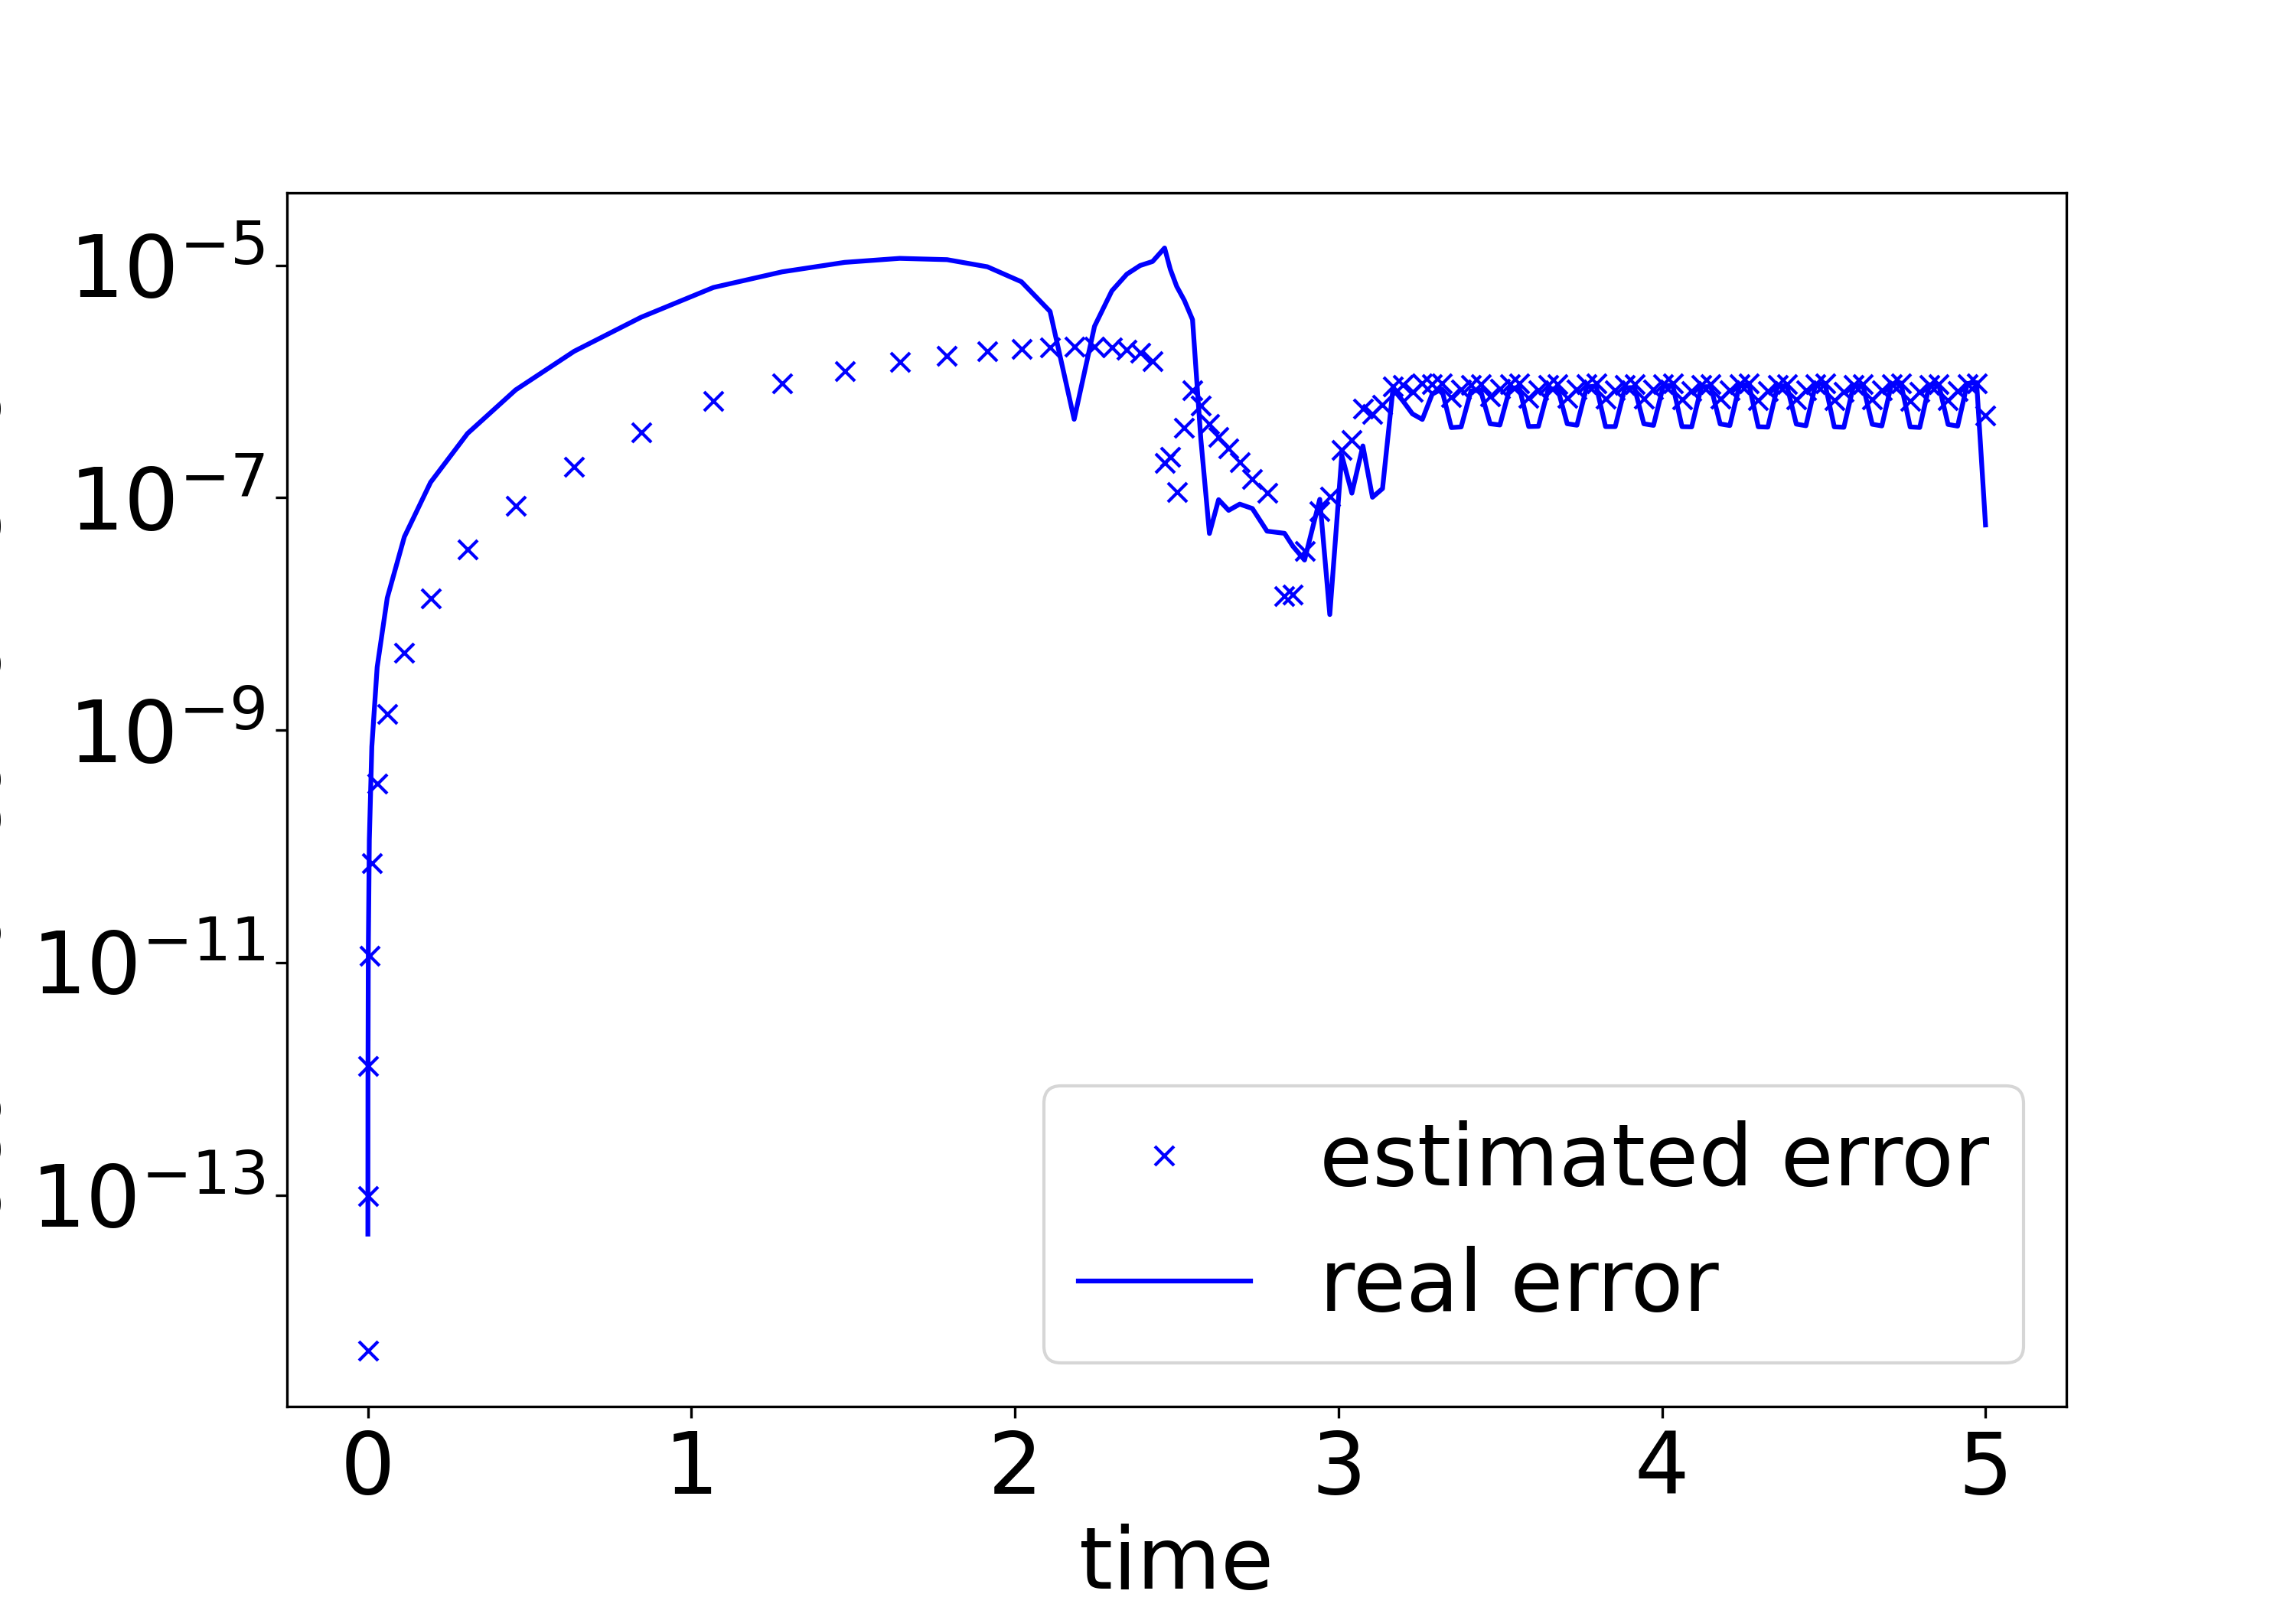
\includegraphics[width=1\textwidth]{images/errorEstimateRKF45.png}
       	\subcaption{\textbf{RKF45}} 
        \label{fig:errorEstimateEvolutionRKF45}
    \end{subfigure}
    \begin{subfigure}{0.32\textwidth}
    	\centering
    	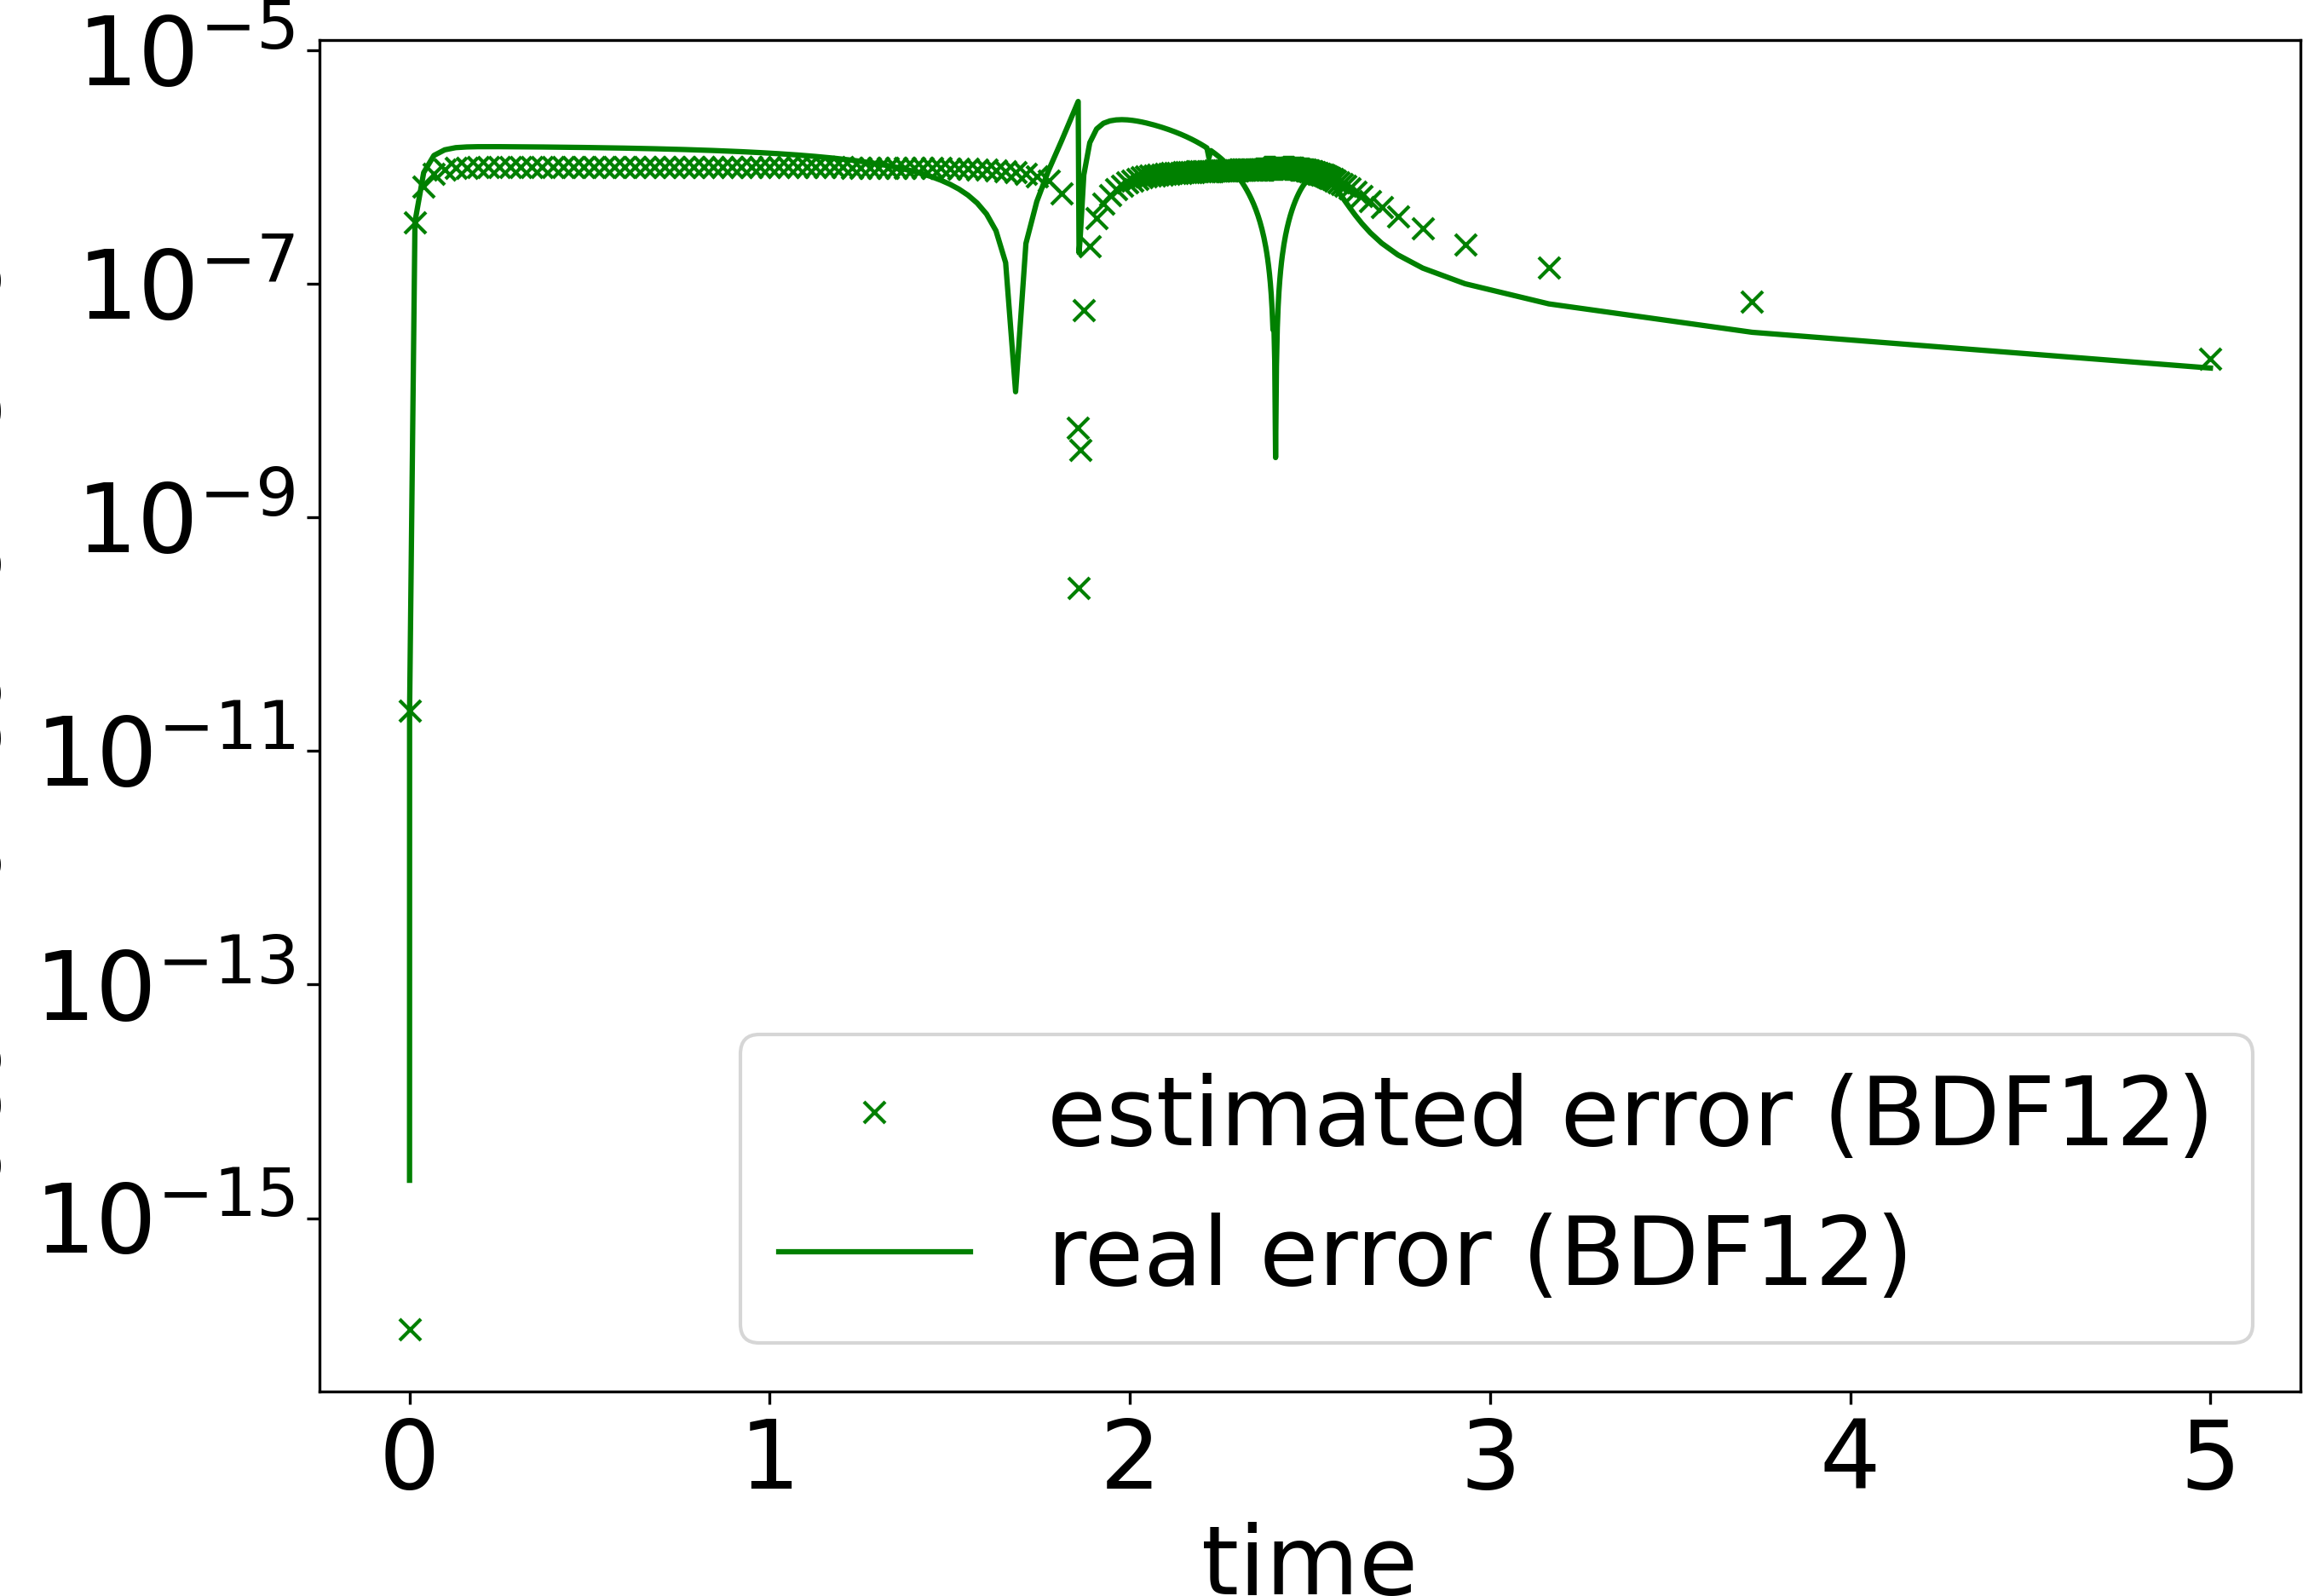
\includegraphics[width=1\textwidth]{images/errorEstimateBDF12.png}
       	\subcaption{\textbf{BDF12}} 
        \label{fig:errorEstimateEvolutionBDF12}
    \end{subfigure}
    \begin{subfigure}{0.32\textwidth}
    	\centering
    	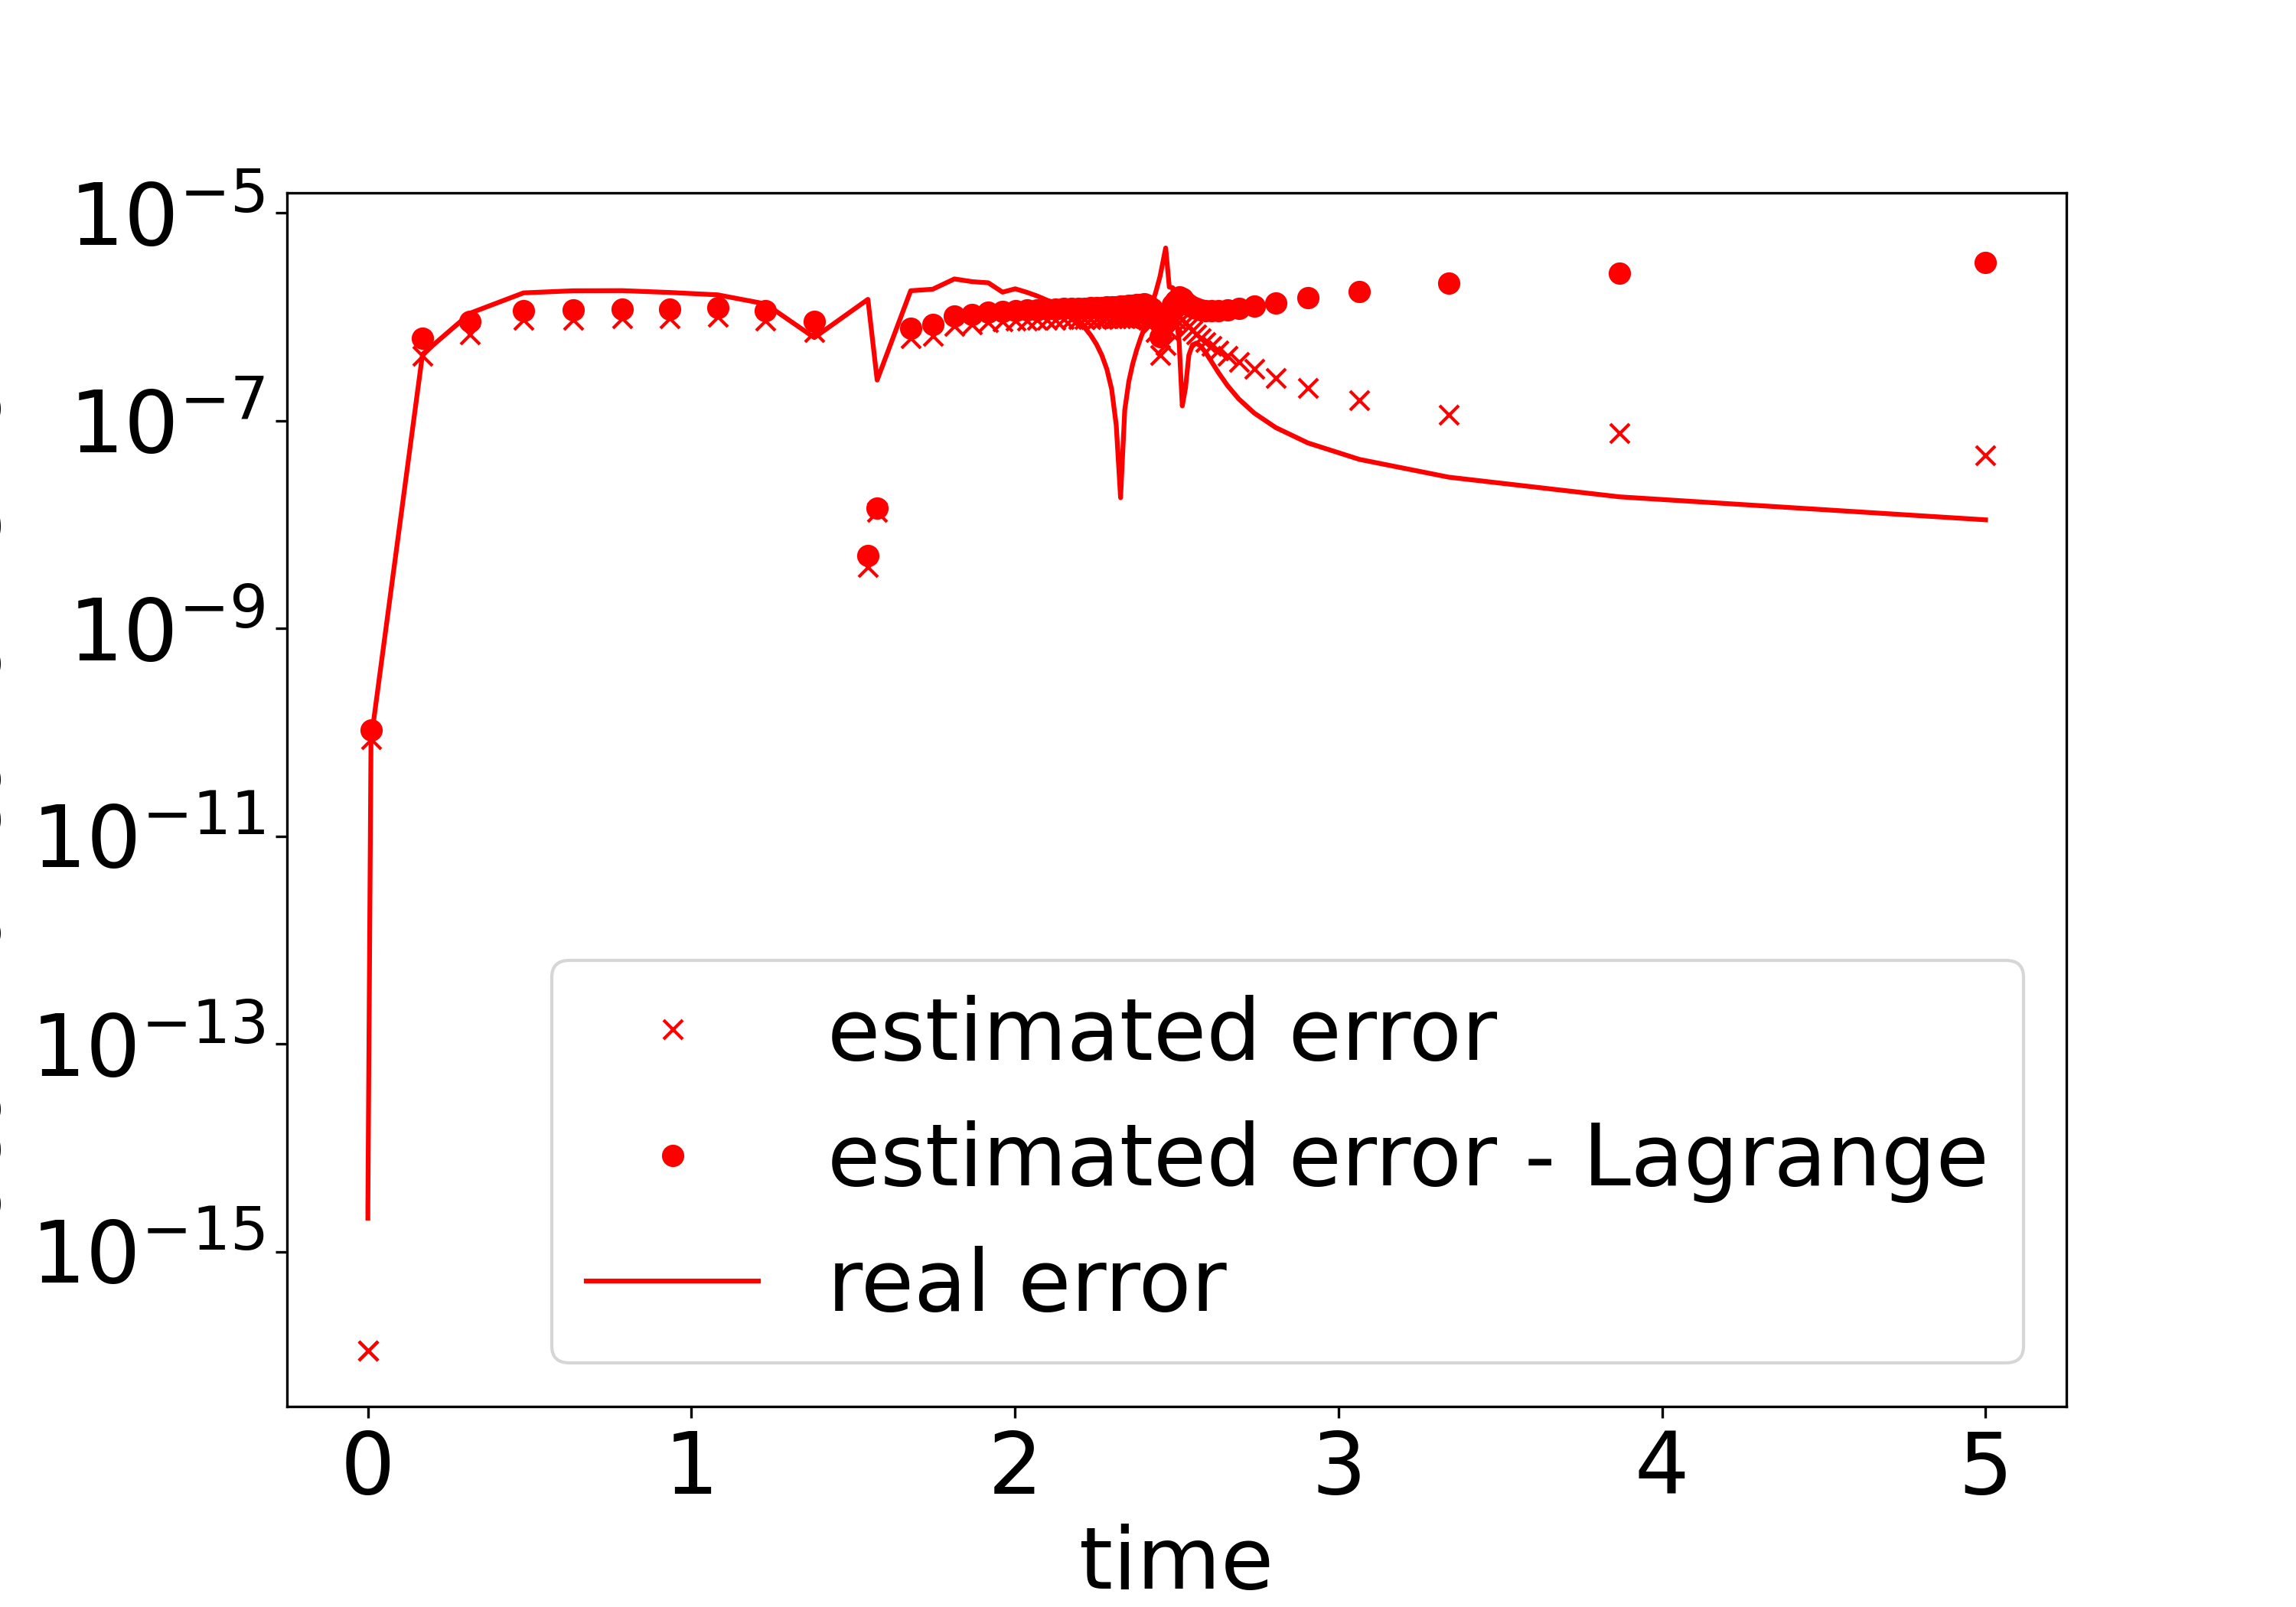
\includegraphics[width=1\textwidth]{images/errorEstimateBDF23.png}
       	\subcaption{\textbf{BDF23}} 
        \label{fig:errorEstimateEvolutionBDF23}
    \end{subfigure}
    \caption{Evolution of the local truncation error and of the error estimate for the single state problem defined in \autoref{eq:first_DAE_algeb} with the implemented numerical schemes}
    \label{fig:errorEstimateEvolutionALL}
\end{figure}

In conclusion, the implicit BDF23 method gives the best results because overall, the induced total error remains low, it allows for the highest timestep sizes and the local truncation error is generally well estimated. In contrast, the BDF12 method is restricted to much smaller timesteps which makes it unattractive for most simulations. Another negative side effect of the small timesteps is the large difference to the analytical solution since the local errors accumulate steadily. The explicit RKF45 fails if the velocity is too high, so it should not be used in such cases. However, it has a strong potential against the BDF23 method for very small velocities because it allows for larger timesteps and in the transition phase from low to high velocities because of the better estimate of the local truncation error.


%\section{Towards a More Physical Model}
%\subsection{Sliding block problem}
%The first considered problem is rather of theoretical nature than of practical relevance with the goal of seismic simulations. A more realistic model with a single variable could be the sliding block problem, in which a block, considered as a point mass, is attached to a spring which moves with constant velocity $V_0$ on a flat surface. The setup is shown in \autoref{fig:sliding_block_graph}. We are interested in the displacement $X$ of the center of mass of the block. The friction between the block and the surface is described by the non-linear law. 
%\begin{figure}[H]
%    \centering
%    \begin{tikzpicture}[scale=2] 
%        \draw[color=black, thick]
%        (1,0) to [short] (5,0){} 
%        (1.2,0.6) to [R,l=$k$,o-](2.8,0.6)
%        to node[short]{}(3,0.6)
%        (3,1.15) to node[short]{}(3,0.05)
%        (3,0.05) to node[short]{}(4.5,0.05)
%        (4.5,0.05) to node[short]{}(4.5,1.15)
%        (3,1.15) to node[short]{}(4.5,1.15)
%        (3.75,0.6) node[]{\large{\textbf{M}}}
%        (1.2,0.8) node[]{$V_0$}
%        ;
%        \draw[<-,color=black, thick] (1.05,0.7) to node[short]{}(1.35,0.7);
%    \end{tikzpicture}
%    \caption{Sliding block problem}
%    \label{fig:sliding_block_graph}
%\end{figure}